\documentclass[twoside,11pt]{article}

% Any additional packages needed should be included after jmlr2e.
% Note that jmlr2e.sty includes epsfig, amssymb, natbib and graphicx,
% and defines many common macros, such as 'proof' and 'example'.
%
% It also sets the bibliographystyle to plainnat; for more information on
% natbib citation styles, see the natbib documentation, a copy of which
% is archived at http://www.jmlr.org/format/natbib.pdf

\usepackage{jmlr2e}
\usepackage{listings}
\usepackage{graphicx}
\usepackage{subfigure}
\usepackage[margin=0.75in]{geometry}
\usepackage{courier}
\usepackage{color}
\usepackage{listings}
\usepackage{algorithm}
\usepackage{algorithmic}
\usepackage{multirow}
\usepackage{rotating}
\usepackage{enumerate}

\definecolor{dkgreen}{rgb}{0,0.6,0}
\definecolor{gray}{rgb}{0.5,0.5,0.5}

\begin{document}

\lstset{language=Matlab,
   keywords={break,case,catch,continue,else,elseif,end,for,function,
      global,if,otherwise,persistent,return,switch,try,while},
   basicstyle=\ttfamily,
   keywordstyle=\color{blue},
   commentstyle=\color{dkgreen},
   stringstyle=\color{red},
   numbers=left,
   numberstyle=\tiny\color{white},
   stepnumber=1,
   numbersep=10pt,
   backgroundcolor=\color{white},
   tabsize=4,
   showspaces=false,
   showstringspaces=false}


% Definitions of handy macros can go here

\newcommand{\dataset}{{\cal D}}
\newcommand{\fracpartial}[2]{\frac{\partial #1}{\partial  #2}}

% Short headings should be running head and authors last names

\firstpageno{1}

\title{Object localization enhancement by multiple segmentations fusion}

\author{\name Ahmed Gad \email amounir@cvc.uab.es \\
       \addr Computer Vision Center\\
       Edificio O, Campus UAB\\
       Bellaterra, 08193, Spain
}

\editor{Ramon Baldrich}

\maketitle

\begin{abstract}

Despite being a very complex task, image segmentation is used as a vital
prerequisite in several computer vision applications, including object tracking,
object recognition and the more challenging object localization. Image
segmentation is known to be unstable and is highly affected by image
perturbations such as shadows, shading and highlights. In our work, we combine
different cues from multiple segmentations of each image to obtain better
segmentations and, hence, better object localization. We propose the
idea of combining multiple segmentations in a bottom up fashion to obtain
enhanced and more reliable image segmentation using the criteria of ``segment
goodness''. We also propose the ``voting'' technique for integrating
image partitions in a top-down fashion to obtain enhanced object localization.
Finally, we discuss some possible extensions for our method that will potentially
boost its performance. Our results exceed the previously published,
state-of-the-art results on a challenging dataset: The PASCAL VOC 2007 object
segmentation challenge.

\end{abstract}

\begin{keywords}
image segmentation, object localization.
\end{keywords}

\section{Introduction}

Image segmentation is a computer vision process where the focus is on
partitioning
an image into a set of non-overlapping regions. This is an extremely challenging
task as on real images, the varying shapes of the objects provoke several
effects
related with the illumination such as shadows, shadings and highlights. These
effects
are one of the main problems that should be solved in order to obtain an
efficient
segmentation.

Image segmentation algorithms can be divided in several ways, however, all of
the
existing approaches can first be divided into two main hierarchies: bottom-up
approaches and top-down approaches.
 
Bottom-up segmentation approaches mainly examine
the image and try to figure out how to divide it into coherent and meaningful
segments. 
Comprehensive surveys as presented by \cite{Yz_colorimage} and
\cite{Cheng01colorimage} 
drew the basis for the current classification of bottom-up segmentation
techniques. 
From all of these existing methods, segmentation methods can be divided into
four 
main categories: feature-based, image-based, physics based and hybrid
approaches.

Feature based approaches mainly focus on the photometric
information of an image represented by its histogram as in the work by
\cite{1059188}
and \cite{Yang07unsupervisedsegmentation}. Image-based approaches
exploit the spatial coherence of colour in an image and an example is given
from the work of \cite{649319}.
Physics-based methods use physics and psychophysics information to perform the
segmentation. Finally, hybrid techniques combine methods of the previous
categories.

Top-down approaches, on the other hand, are guided
primarily by high-level information and the use of class-specific criteria. The
motivation
for using these class-specific criteria, as shown by \cite{649285}, has two parts.
The first is that although recent image segmentation algorithms provide
impressive
results, they still often fail to capture meaningful and at times crucial parts
of the objects in the image. The second is that these
methods are analogous to human vision in the sense of indicating high-level,
class-based criteria to segment the images in a meaningful manner. Examples of
using top-down approaches to perform segmentation are shown in the work of
\cite{649285}, \cite{Leibe04combinedobject}, \cite{1097721} and \cite{163215}.

The importance of image segmentation has been shown in a variety of computer
vision problems. In other words, a robust and efficient segmentation is usually
an important preprocessing step for several computer vision tasks such as object
tracking or object recognition. However, extensive experiments by
\cite{Unnikrishnan_2007_5789}
show that when using a single region generated by an image segmentation
algorithm, the
segmentation quality is highly variable and dependant on image data, the
segmentation algorithms and the parameters used to create this segmentation.
This was a motivation for the emerging new trend in object
recognition that uses the segments generated from multiple
segmentation algorithms and tries to merge them efficiently to recognize objects
in the scene \cite{Efros_2006_5395}, \cite{PSH08} and \cite{malisiewicz-bmvc07}.

This trend of using multiple segmentations was also our motivation in our work.
In our work we focus on
two parts. The first one is building a robust and efficient
segmentation method that uses the
information provided by several other segmentation algorithms to build
more reliable image segmentations in a bottom-up fashion. The second is
using this new segmentation along with the other segmentation
results to recognize and localize objects in the image by performing object
class segmentation to this image then combining the localization results in
a top-down approach.

The goal of object class image segmentation is to produce
a pixel-level segmentation of the input image. In figure \ref{fig:obj_seg} we
show
an example of object class image segmentation. This is a higly constrained
problem where most state-of-the-art approaches focus on exploiting contextual
information available around each pixel. Afterwards, they measure feature
statistics from this information (in this case histograms of visual words)
and use the bag-of-words technique in order to determine the class that
each pixel falls into.

\begin{figure}[!t]
\centering
\subfigure[] {
    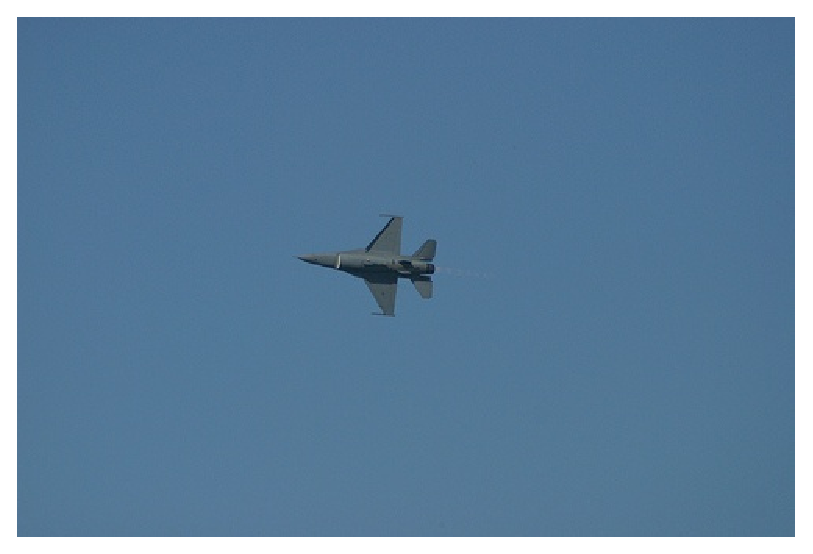
\includegraphics[width=115pt,height=80pt]{./Figures/forg1.eps}
    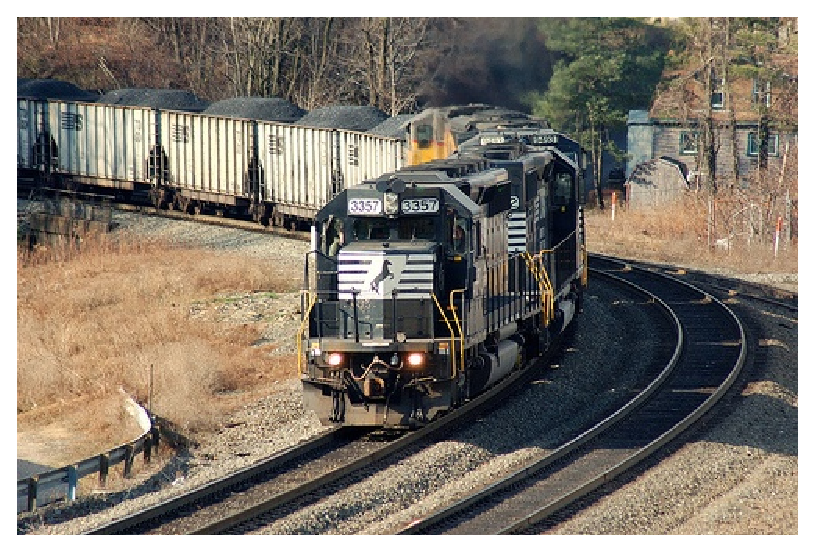
\includegraphics[width=115pt,height=80pt]{./Figures/forg2.eps}
    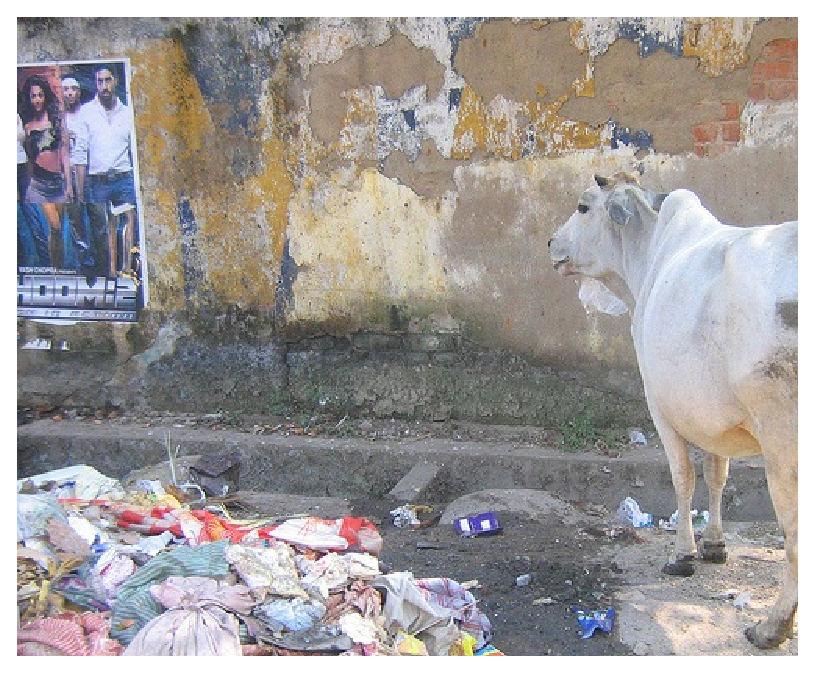
\includegraphics[width=115pt,height=80pt]{./Figures/forg3.eps}
    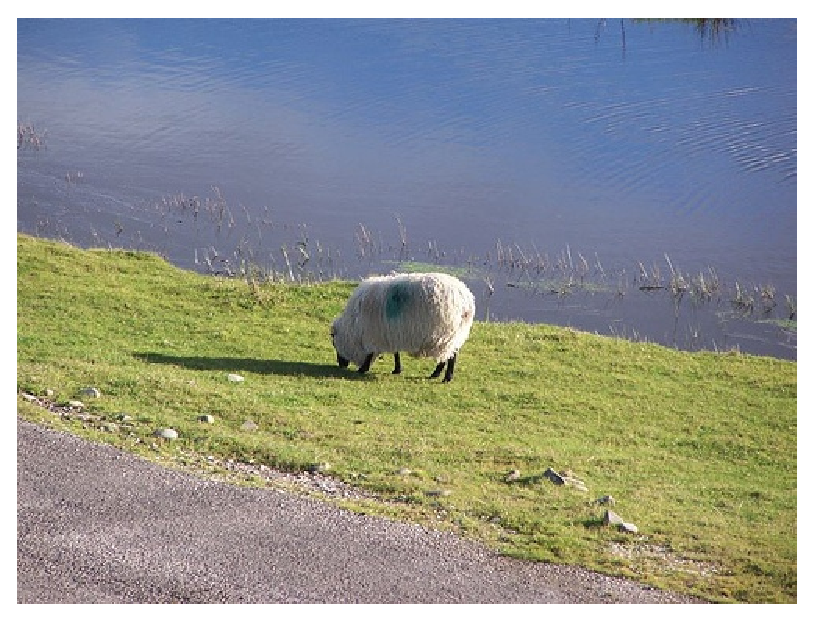
\includegraphics[width=115pt,height=80pt]{./Figures/forg4.eps}
    \label{fig:classsegorg}
}\\
\subfigure[] {
    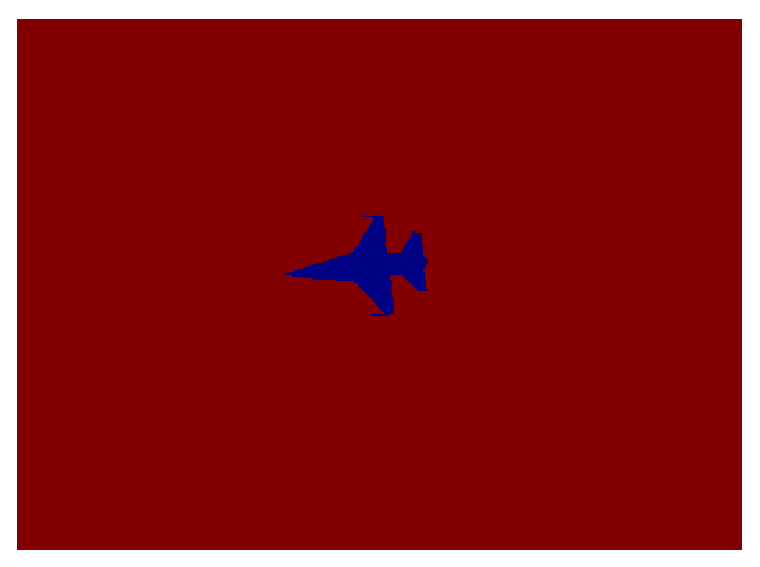
\includegraphics[width=115pt,height=80pt]{./Figures/gt1.eps}
    
\includegraphics[width=115pt,height=80pt]{./Figures/gt2.eps}
    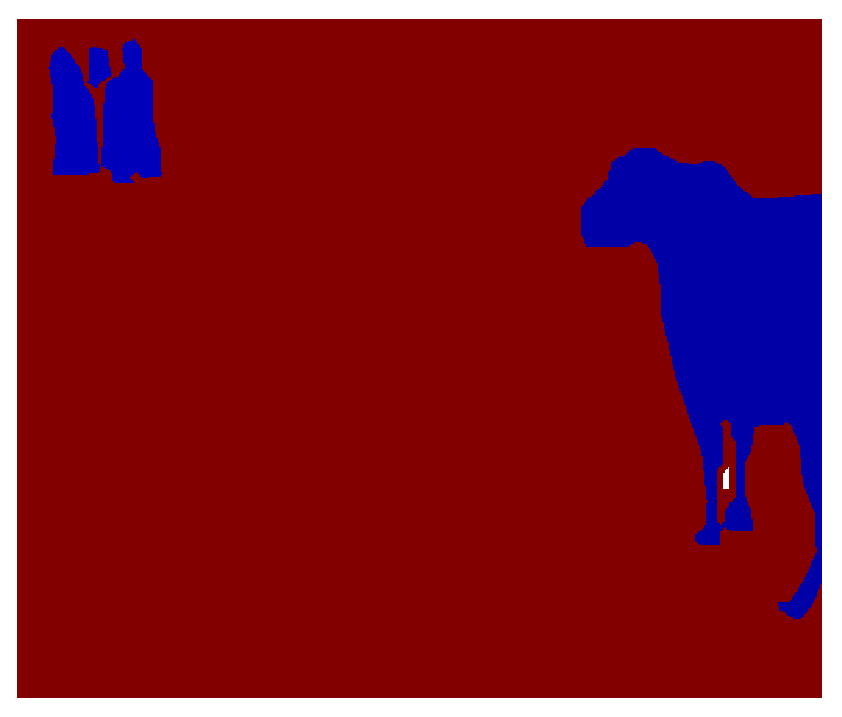
\includegraphics[width=115pt,height=80pt]{./Figures/gt3.eps}
    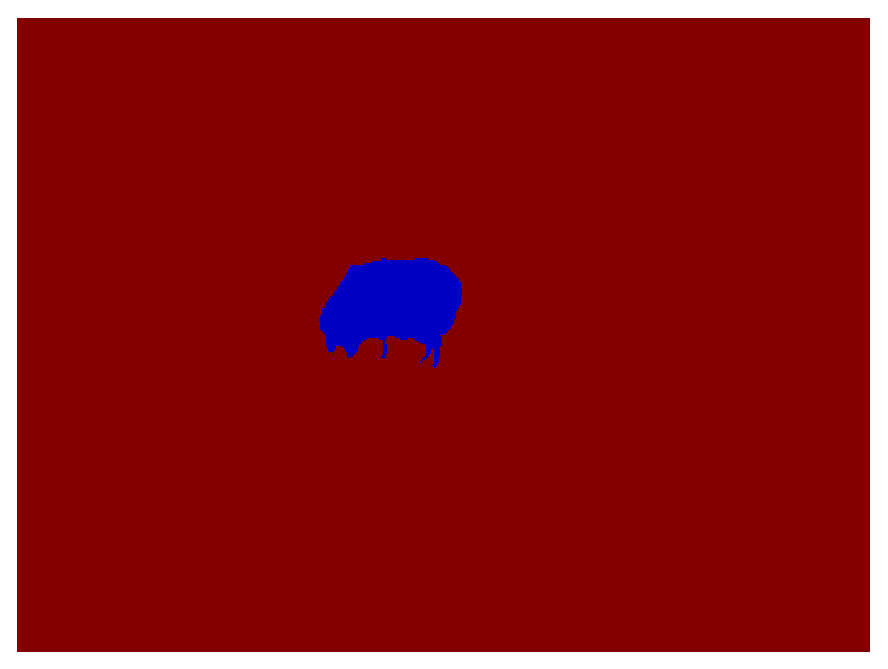
\includegraphics[width=115pt,height=80pt]{./Figures/gt4.eps}
    \label{fig:classseggt}
}\\
\subfigure[] {
    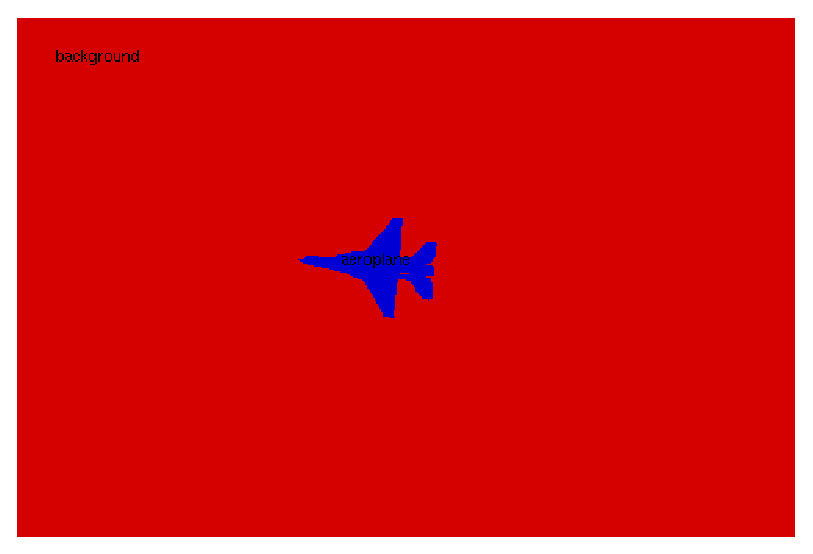
\includegraphics[width=115pt,height=80pt]{./Figures/vcrf1.eps}
    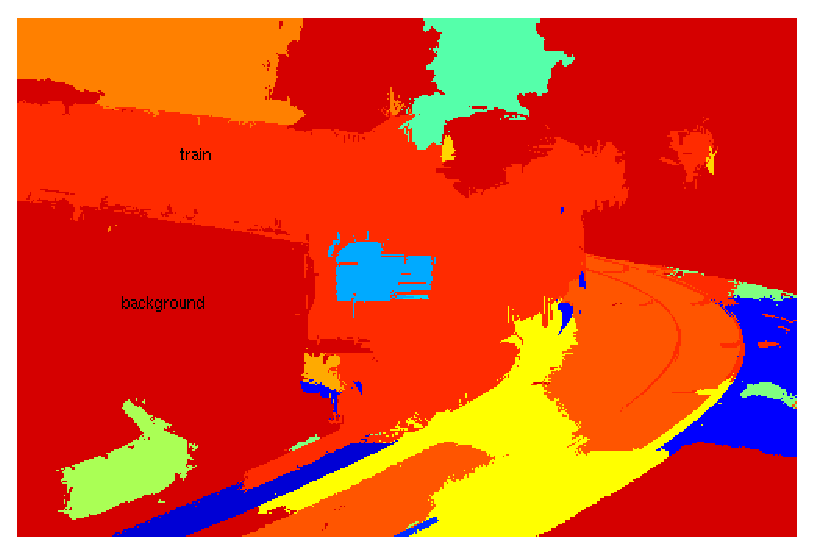
\includegraphics[width=115pt,height=80pt]{./Figures/vcrf2.eps}
    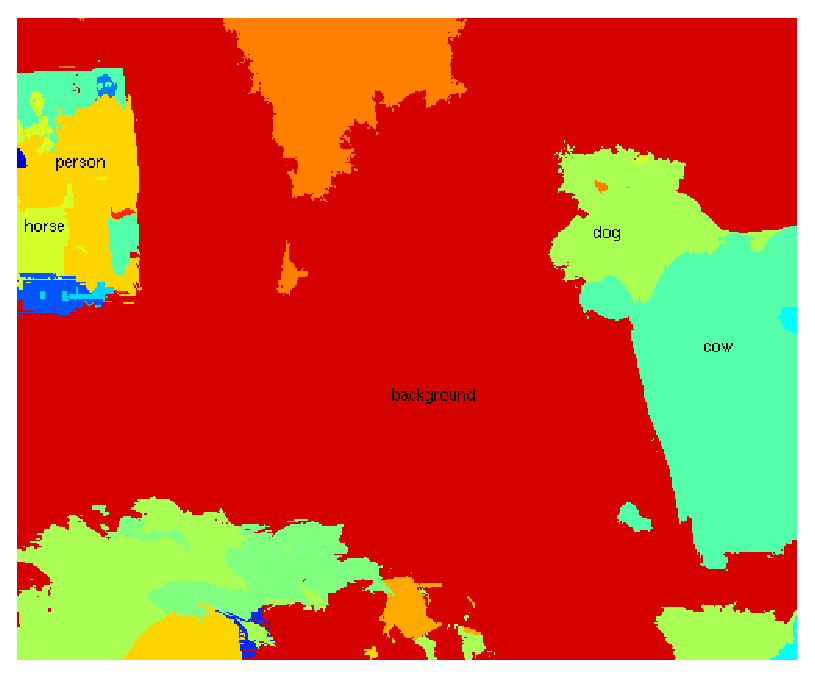
\includegraphics[width=115pt,height=80pt]{./Figures/vcrf3.eps}
    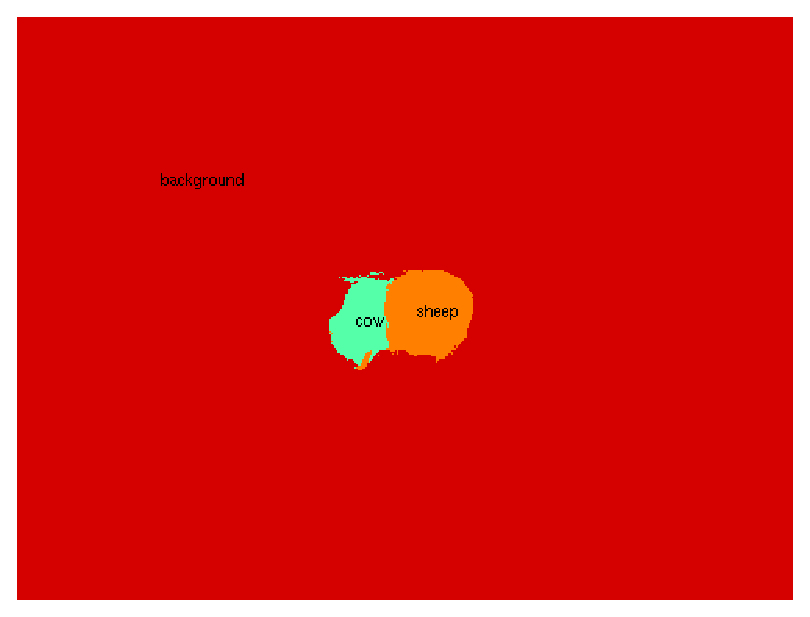
\includegraphics[width=115pt,height=80pt]{./Figures/vcrf4.eps}
    \label{fig:classsegres}
}
\caption{(a) Original images (b) Ground truth
(c) Obtained object class segmentation}
\label{fig:obj_seg}
\end{figure}

Instead of working on pixels, \cite{fulkerson09class} present a method to
perform
object class segmentation by aggregating the histograms in the neighbourhood of
the small regions obtained from a conservative oversegmentation, or
``superpixels''
as described by \cite{Ren03learninga} and \cite{4587471} as their elementary unit
of
any detection, categorization or localization scheme. They not only use the
information obtained from superpixels but also they use of neighbouring
superpixels to provide more contextual information. However, in our work we show
that even when adding neighbourhood information, superpixels are still not
the best choice for describing an object.

In our work, instead of using pixels or superpixels, we use regions emerging
from several segmentation techniques. Our results show that even superpixels
do not capture enough information about the objects being recognized and
localized that can be better captured by using larger segments.
We learn a model from each segmentation method
to classify the regions of this segmentation method. Afterwards, we combine
all of the results coming from each model separately into a new model by the
technique that we call, the ``voting technique''. Our results show that
combining
results from outputs of several classifications give a significant improvement
over using each classification solely. The results are even better than those
obtained while using superpixels with joining neighbourhood information for
classification.

This thesis is organized as follows. In section 2, we highlight some of the
existing
literature in the field of segmentation and object recognition and localization.
We then explain more details about the segments neighborhood in section 3 which is the
core of the class segmentation method of \cite{fulkerson09class}. It is also
considered as the basis of our method. In section 4, we thoroughly illustrate
our core approach. In section 5, we show the performed experiments and the results we
have. In Section 6 we sum up our work with some conclusions. Finally, in section 7
we introduced some of the extensions of our method that will potentially improve
its performance.

\section{Related Work}

\begin{figure}[!t]
\centering
\subfigure[] {
    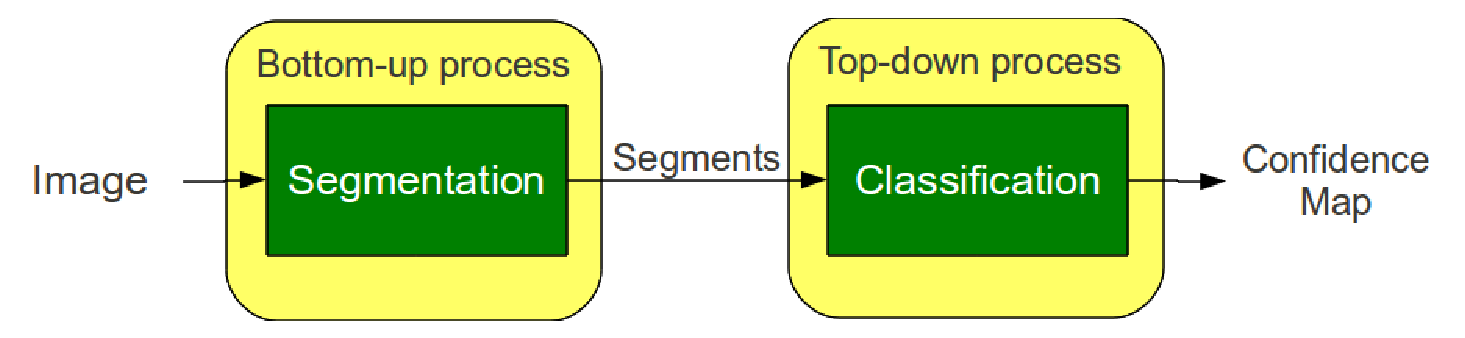
\includegraphics[width=345pt,height=60pt]{./Figures/org_framework.eps}
    \label{fig:framework_org}
}\\
\subfigure[] {
    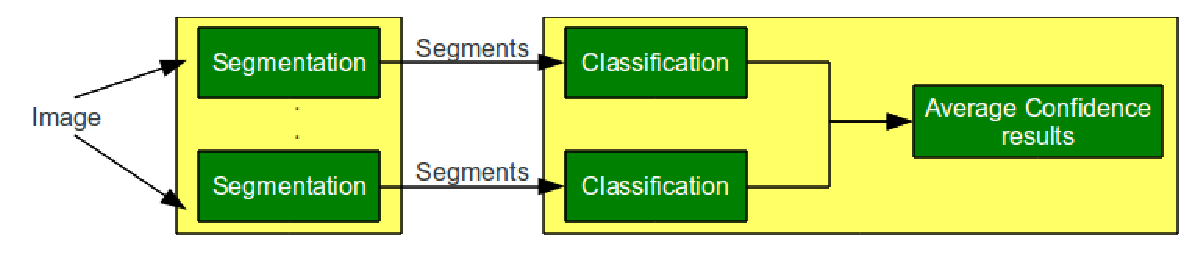
\includegraphics[width=365pt,height=65pt]{./Figures/cordelia_framework.eps}
    \label{fig:framework_cordelia}
}\\
\subfigure[] {
    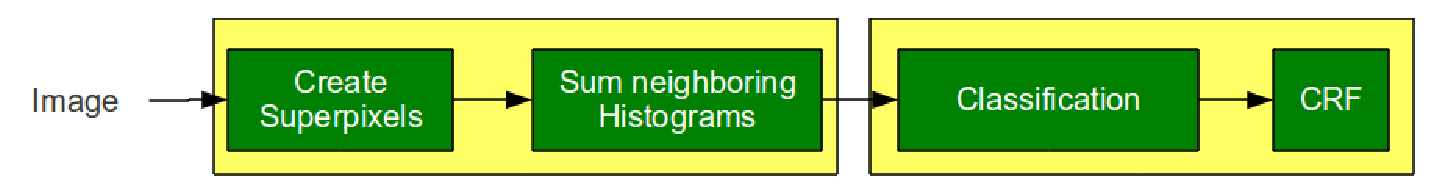
\includegraphics[width=365pt,height=40pt]{./Figures/fulkerson_framework.eps}
    \label{fig:framework_fulkers}
}
\caption{Object class segmentation frameworks (a) Basic framework (b) \cite{PSH08} framework
(c) \cite{fulkerson09class} framework}
\label{fig:obj_seg_model}
\end{figure}

In this section we briefly explain the existing literature in addressing the
problems we are proposing in our work. We are addressing two different problems:
First, the segmentation problem. We are building a new segmentation method
based on segments coming from different other segmentations by combining these
segments in a bottom up fashion. Second, the
recognition problem. We are performing object class image segmentation which
is the process of producing a pixel level segmentation for the whole image.
In other words, recognizing which class does every pixel of the image
lies into. Figure \ref{fig:framework_org} shows the basic framework used
to produce an object class image segmentation.

\subsection{Image segmentation}

The problem of image segmentation has been the subject of considerable research
activity
over the last decades. The aim of image segmentation is to identify the
homogeneous
regions in the image. In other words, it is the process of partitioning an image
into
a set of disjoint and homogeneeous regions. This task can be equivalent to the
task of
identifying boundaries between the regions.

Segmentation is an extremely important preprocessing task for several
applications of
image processing and computer vision. It represents the first step of low-level
processing of imagery. Consequently, many literature exist trying to address the
segmentation problem. Existing segmentation methods can be divided into two
main sections. Top-down and bottom-up segmentation techniques.

According to the color image segmentation survey by \cite{Yz_colorimage},
existing bottom-up segmentation methods can be divided into feature space-based,
image-domain based, physics-based and hybrid techniques.

According to \cite{Yz_colorimage}, feature space based techniques rely on the
following observation. ``If we assume that color is a constant property of the 
surface of each object within an image and we map each pixel of the color image
into a certain color space, it is very likely that different objects present in
the image will manifest themselves as clusters or clouds of points.'' An example
of the techniques that are considered as feature-based is the clustering.
Clustering
can be defined as a non-supervised classification process where one has to generate
classes or partitions without any prior information. \cite{Shi_2000_3808} consider
image segmentation as a clustering problem via graph partitioning.

Another way to approach the image segmentation problems is to use the image
domain based techniques. According to \cite{Yz_colorimage} existing
techniques
are divided into split-and-merge, region growing, edge based and neural network-based
techniques. One of the most commonly used image based techniques for image
segmentation is the one introduced by \cite{Felzenszwalb04efficientgraph-based}.
They define a predicate for measuring the evidence for the boundary between two
regions using a graph based representation of the image. Afterwards, they
develop an efficient segmentation algorithm based on this predicate.

Physics based techniques, the proposed methods focus on
analyzing how light interact with coloured materials and try to introduce
models of this physical interaction in the segmentation algorithms. A
milestone in physics-based segmentation was the ``dichromatic reflection
model'' introduced by \cite{136817}.

Finally, hybrid methods focus on combining the previous techniques together.
An example of using hybrid techniques for performing segmentation is the work
presented in this thesis. The method proposed focuses on getting the
best segments out of several bottom up segmentation methods of different
categories and tries to combine them together.

Top-down segmentation algorithms, also known as class-specific
segmentation algorithms, were developed to overcome the difficulties in
low-level segmentation. Mainly, they add more semantics to the top-down
segmentations by grouping segments that belong to the same object based
on some prior information about the
characteristics of the object. The work by \cite{649285} and \cite{1097721}
provide an example for top down segmentation algorithms.

Moreover, several approaches also exist that combine bottom-up with top-down cues
to yield a better segmentation. An example is the work by \cite{Levin06learningto}.
They train a fragment based segmentation algorithm which
takes into account both bottom up and top down cues simultaneously. They formulate
the problem in the framework of conditional random fields and derive a feature
induction algorithm for CRF which allows it to efficiently search over thousands
of candidate fragments.

\subsection{Objects recognition and localization}

Recently, significant progress has been made in image-level object
categorization. The ``classification'' task works on a certain image and tries
to determine whether it
contains at least a single instance of a certain object or not. The bag of words
approach proved to be a suitable technique for this task. However, this
image level object categorization fails to determine spatial information about
the objects. This led to significant interest on the related fronts of
localization and pixel-level categorization. Challenges like PASCAL VOC
classification, detection and segmentation encourage further research in
object recognition and localization.

Sliding window classifiers have been well explored for the task of detecting
the location of an object inside an image. \cite{Lampert08beyondsliding} propose
a simple yet powerful branch-and-bound scheme that allows efficient maximization
of a large class of classifier functions over all possible subimages. Their
method works in sublinear time and is applicable to object detection and
retrieval. \cite{1478410} perform bag of features classification within a local region.
However, the size of the region is fixed (rectangular window).

Moreover, many approaches exist to class segmentation which work at the pixel
level or more local features like textons as the work by
\cite{Shotton06textonboost:joint}. \cite{bb32196} construct semantic forests for
extremely fast classification.

The basis of our work is the work of \cite{fulkerson09class} and
\cite{PSH08}. \cite{fulkerson09class} advocate the use of superpixels as the
basic unit of their class segmentation or localization scheme. They construct
a classifier on the histogram of local features found in each superpixel. They
regularize this classifier by aggregating histograms in the neighborhood of each
superpixel. Finally,
they refine their results by using a classifier in a conditional random field
operating on the superpixel graph. Figure \ref{fig:framework_fulkers} shows
a graphical explanation for \cite{fulkerson09class} framework.

\cite{PSH08} works similarly to that of \cite{fulkerson09class}. The difference is
that it extracts superpixels like objects by intersecting multiple segmentations and
then classifies them by averaging the classification results from
all of the member regions. A clearer explanation is shown in figure
\ref{fig:framework_cordelia}. The work of \cite{fulkerson09class} provides the insight
for our method. We explain it in more details in the next section.

\section{Segment neighbourhoods}

\cite{fulkerson09class} introduced the concept of superpixel
neighbourhoods. They note  that superpixels by their nature do not
carry any meaningful information about the object where they are contained.
However, establishing a relation between the superpixel and its neighbour helps
make the superpixel more meaningful.

They assume the superpixels in an image form a graph $G(S, E)$ where
superpixels $s_i \epsilon S$ are considered the nodes of the graph, $E$ is the set
of edges formed between pairs of adjacent superpixels ($s_i$, $s_j$) in the
image.

Let $D(s_i, s_j)$ be the length of the shorteset path between two superpixels.
In this case, $H_i^N$ is the histogram obtained by merging the histograms of the
superpixel $s_i$ and neighbours who are less than N nodes away in the graph

\begin{equation}
\label{eq:one}
H_i^N = \sum_{s_j|D(s_i,s_j)\leq{N}} H_j^0.
\end{equation}

\cite{fulkerson09class} use the histogram obtained from equation 1
for the classification. They use different values of $N$ to construct the histograms.
This means, \cite{fulkerson09class} assume that increasing the value of $N$ means
considering the histogram resulting from a larger segment instead of individual
superpixels. This segment is constructed by the value of $D$ which is the shortest
path between two superpixels and is calculated from the minimum difference of
colours of each two neighboring superpixels.

We also tried using the same concept but for joining segments instead of superpixels. 
This concept improved some of the segmentations like the mean-shift and the
graph based. On the other hand, joining segments by summing the neighbour's
histograms got worse results for some other segmentations like the
normalized-cut. From these observations we concluded that joining segments don't
always work. Sometimes when the segment is already large, joining the segments makes
them carry other useless information from other different objects. In this
case, the results start decreasing gradually.

In figure \ref{fig:neigh_effect}, we see the effect of increasing the value of 
the pixels neighbourhood on the final accuracy of the segmentation.
We conclude that when the
segments are larger and carrying more information, the classification results
are improved. However, the segments should only be merged with other segments
that correspond to the same object. Otherwise, further increasing
of the size of segments, the accuracy tends to decrease dramatically.

\begin{figure}
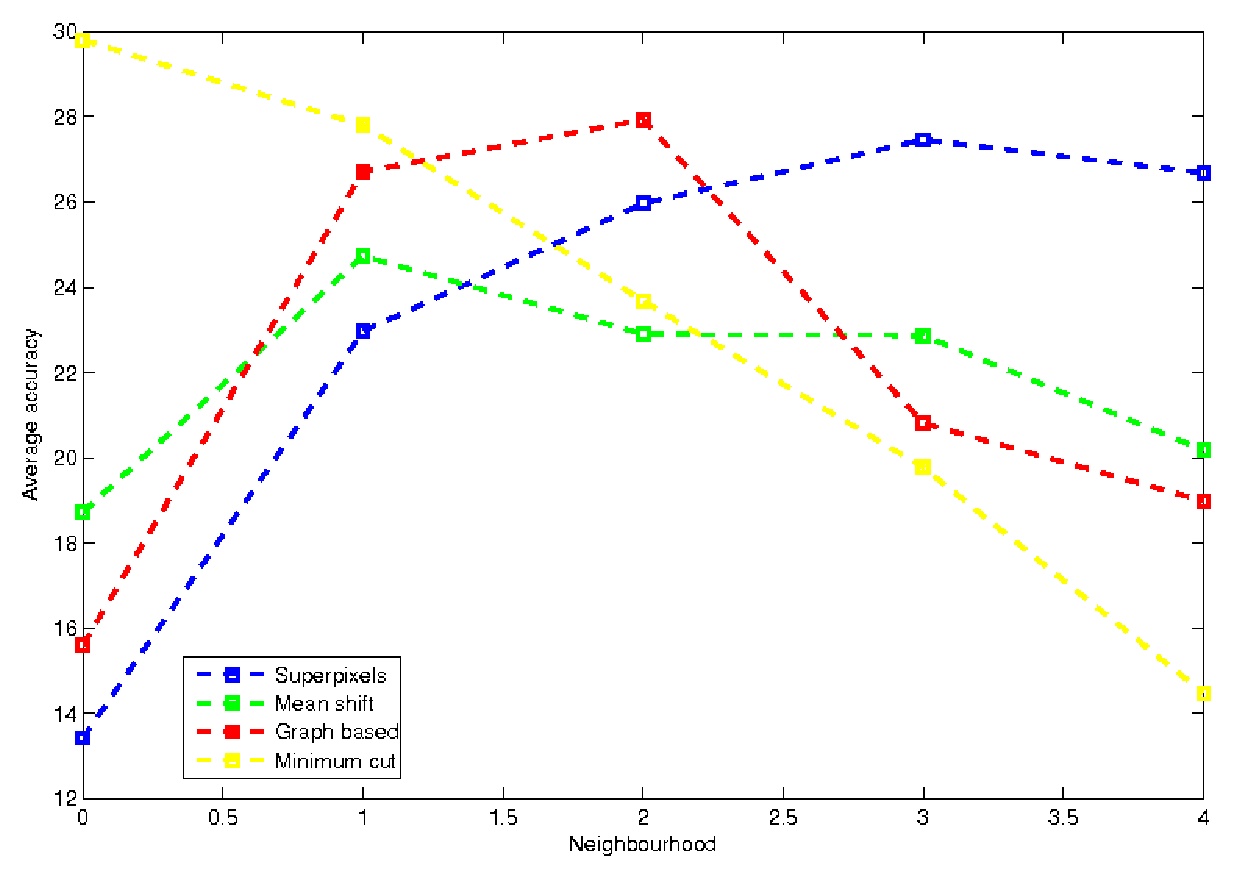
\includegraphics[scale =.65]{./Figures/neigh_acc.eps}
\centering
\caption{Effect of neighbourhood on the average accuracies}
\label{fig:neigh_effect}
\end{figure}


From these conclusions we arrive at our insight for obtaining better segmentations
that can help in improving the object localization consequently. We first have to
favor large segments from all segmentations. These segments are more meaningful about
the objects and help the classifier to know a better clue about each class of objects.
However, these segments should still be meaningful. In other words, they should be
good segments. We provide a definition of ``goodness'' for segments in later
sections.

\section{Core approach}

\begin{figure}[!t]
\centering
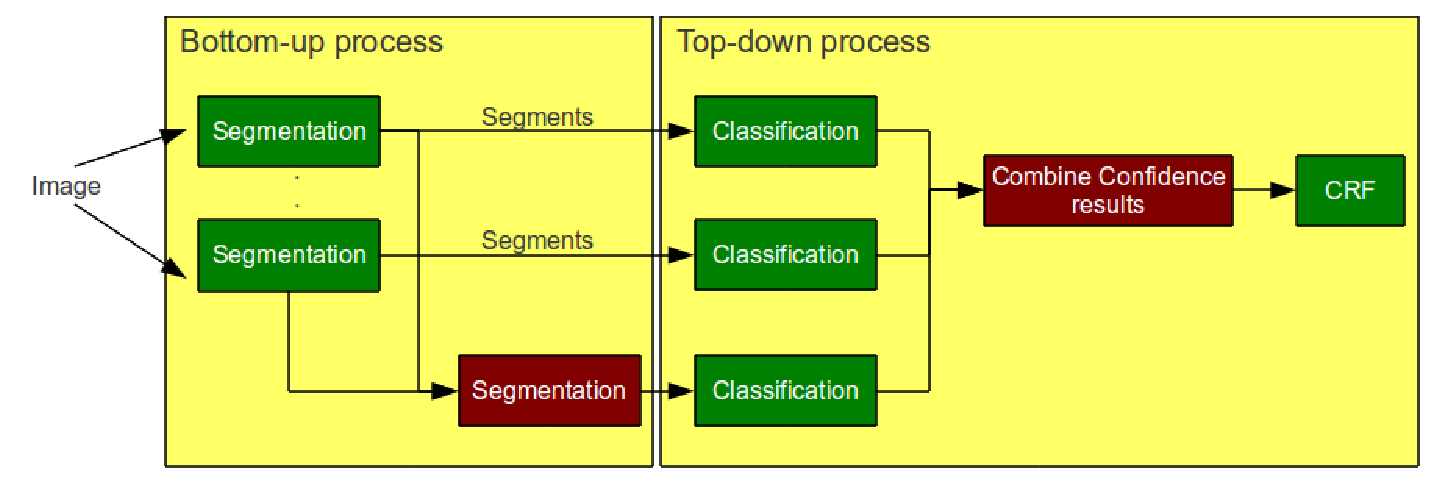
\includegraphics[scale=0.7]{./Figures/our_framework.eps}
\caption{Our object class segmentation model. Our contributions are highlighted in red.}
\label{fig:our_obj_seg_model}
\end{figure}

In this section, we describe the core of our approach for the object class
segmentation problem. The process involves five main steps. First, we
generated multiple segmentations for each image in our dataset. Second, we use
these segmentations to build a more reliable segmentation. We tried several
techniques to combine these segmentations together into a better final
segmentation.
We'll describe each of these techniques in the next sections.Third, we describe
and classify each region from every segmentation technique including our
generated
segmentation. Afterwards, we combine the regions' classifications into an object
map
indicating which class does each of the pixels lie in. Finally, we refine our
results with a conditional random field. A graphical explanation of our
object class segmentation framework is explained by figure \ref{fig:our_obj_seg_model}

\subsection{Generating multiple segmentations}

Every image segmentation technique uses unique cues to construct segments cues that
differ from those used by other segmentation methods.
In order to build a more reliable segmentation, we constructed a number of
segmentations each containing a number of properties that we desire in our final
segmentation and that are not obtained from a single segmentation method solely.

We generate a segmentation based on mean-shift by \cite{Comaniciu02meanshift}.
In this segmentation we guarantee that the segments mainly vary in the colour
distribution along the whole segment. We also generate another segmentation based
on the graph-based method by \cite{Felzenszwalb04efficientgraph-based} to
guarantee a variation along the edges and we generated a segmentation based on
minimum cut by \cite{Shi_2000_3808} for a specific number of segments to guarantee
some large segments.

Using these segmentations, we obtain mose of the qualities that we desire in our
final segmentation result so that when we mix them we will get a better final
segmentation.

In figure \ref{fig:allsegs} we show an image segmented using all different
segmentations and we show the number of segments generated by each segmentation
method. Our goal now is to first, combine these segmentations in a bottom-up fashion
to obtain a new more reliable segmentation. Second, combine all these segmentations
in a top-down fashion into a better, final object class segmentation.

\begin{figure}[!t]
\centering
\subfigure[] {
    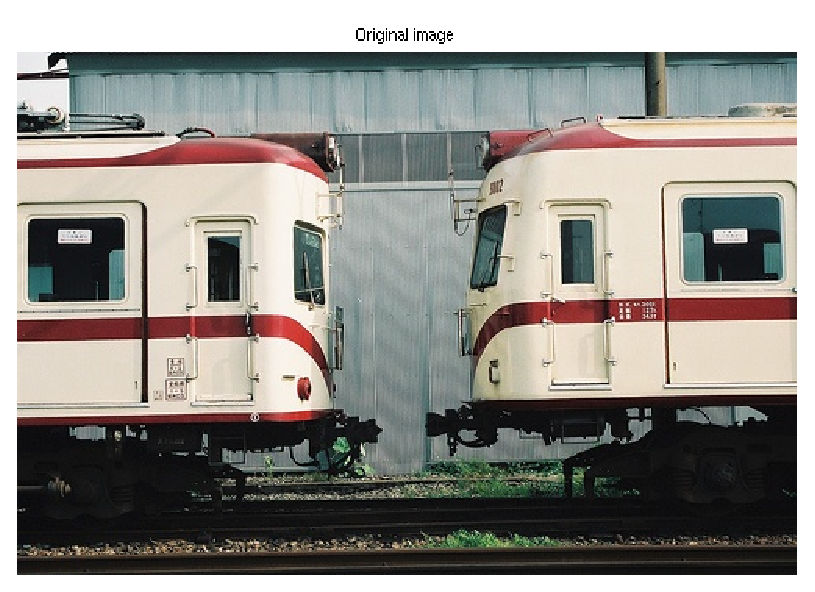
\includegraphics[width=115pt,height=80pt]{./Figures/ORG2.eps}
    \label{fig:org2}
}
\subfigure[] {
    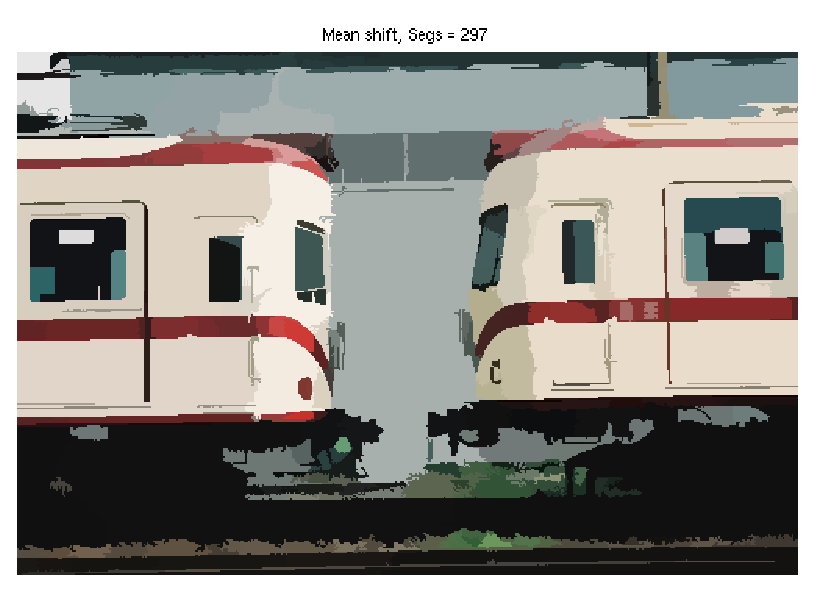
\includegraphics[width=115pt,height=80pt]{./Figures/MS2.eps}
    \label{fig:ms2}
}
\subfigure[] {
    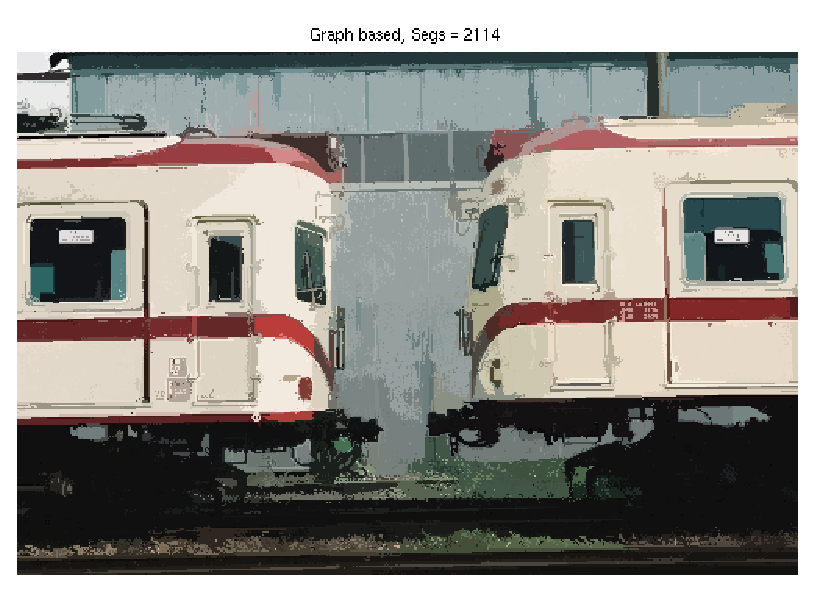
\includegraphics[width=115pt,height=80pt]{./Figures/GB2.eps}
    \label{fig:gb2}
}
\subfigure[] {
    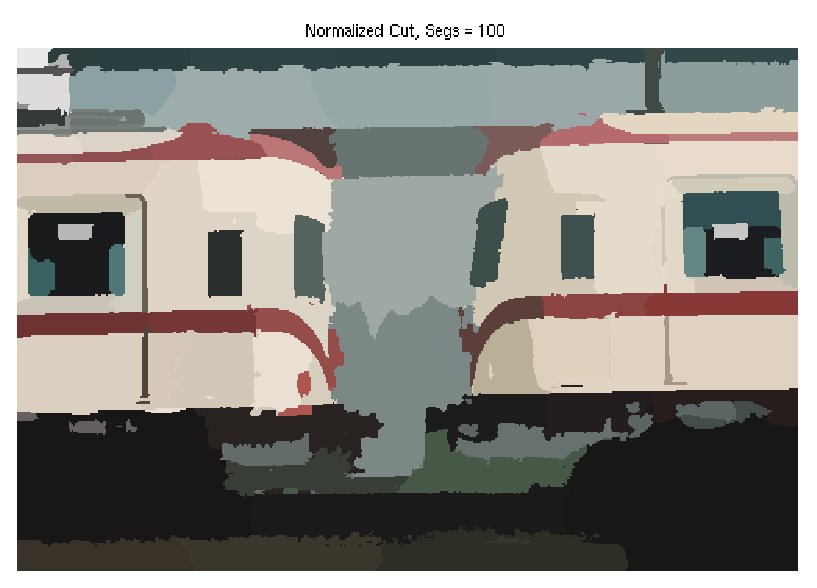
\includegraphics[width=115pt,height=80pt]{./Figures/NC2.eps}
    \label{fig:nc2}
}
\caption{(a) Original image (b) Image segmented using mean shift. Number of
segments = 297 (c) Image segmented using Graph Based technique by
\cite{Felzenszwalb04efficientgraph-based}. Number of segments = 2114 (d) Image
segmented using normalized cut. Number of segments = 100}
\label{fig:allsegs}
\end{figure}

\subsection{Building a more reliable segmentation}

After obtaining different segmentations for each image, we use these
segmentations to build a more reliable segmentation. Our aim is to select
those segments that are considered good enough and split those which aren't
based on some other cues.

Assume we have $N$ segmentations $S_i$, where $i = 1, ..., N$ and each of the
segmentations correspond
to $S_i = \bigcup_{j=1}^{C_i}T_j$, where $T$ is a segment in the segmentation $S$ and $C$
is the number of segments inside
a certain segmentation. We want to build a final segmentation $S^* =
\bigcup_{k=1}^{C^*}T_k^*$
based on the two observations we had before:

\begin{enumerate}
\item
The segments of the final segmentation should be as large as possible. In other
words, we need to minimize
$C^*$
\item
The segments should be ``good'' segments. In our context, we defined a ``good
segment'' as the largest set of connected pixels that lie in the same class and are
coherent in the colour distribution.
\end{enumerate}

Consequently, our motivation for the mixing problem was to start looking for the
large segments and then check if this segment is a valid segment or not. we
tried two techniques to
combine segments. The two techniques perform greedily favoring the largest
segment. The techniques
are described by algorithms \ref{alg:mixall1} and \ref{alg:mixall2}.

\begin{algorithm}
\caption{mix\_all\_segmentations(ip\_img, curr\_segment, all\_segs)}
\label{alg:mixall1}
\begin{algorithmic}
\STATE [largest\_seg, seg\_id] = get\_largest\_segment(ip\_img, all\_segs);
\IF {good\_segment(largest\_seg)}
\STATE include\_segment(seg\_im, largest\_seg);
\ELSE
\STATE include\_segment(seg\_im, mix\_all\_segmentations(largest\_seg, all\_segs
- seg\_id));
\ENDIF
\STATE include\_segment(seg\_im, mix\_all\_segmentations(ip\_img - largest\_seg,
all\_segs));
\RETURN seg\_im;
\end{algorithmic}
\end{algorithm}

\begin{algorithm}
\caption{mix\_all\_segmentations(ip\_img, all\_segs)}
\label{alg:mixall2}
\begin{algorithmic}
\STATE Add all segments from all segmentations to a heap;
\WHILE {! empty(segments\_heap)}
\STATE segment T = largest\_segment()
\IF {segment contains pixels already in the final segmentation}
\STATE remove those pixels
\STATE add the segment again to the heap
\ELSE
\IF {good\_segment(T)}
\STATE include in the final segmentation
\ELSE
\STATE discard this segment
\ENDIF
\ENDIF
\ENDWHILE
\RETURN seg\_im;
\end{algorithmic}
\end{algorithm}
\begin{figure}
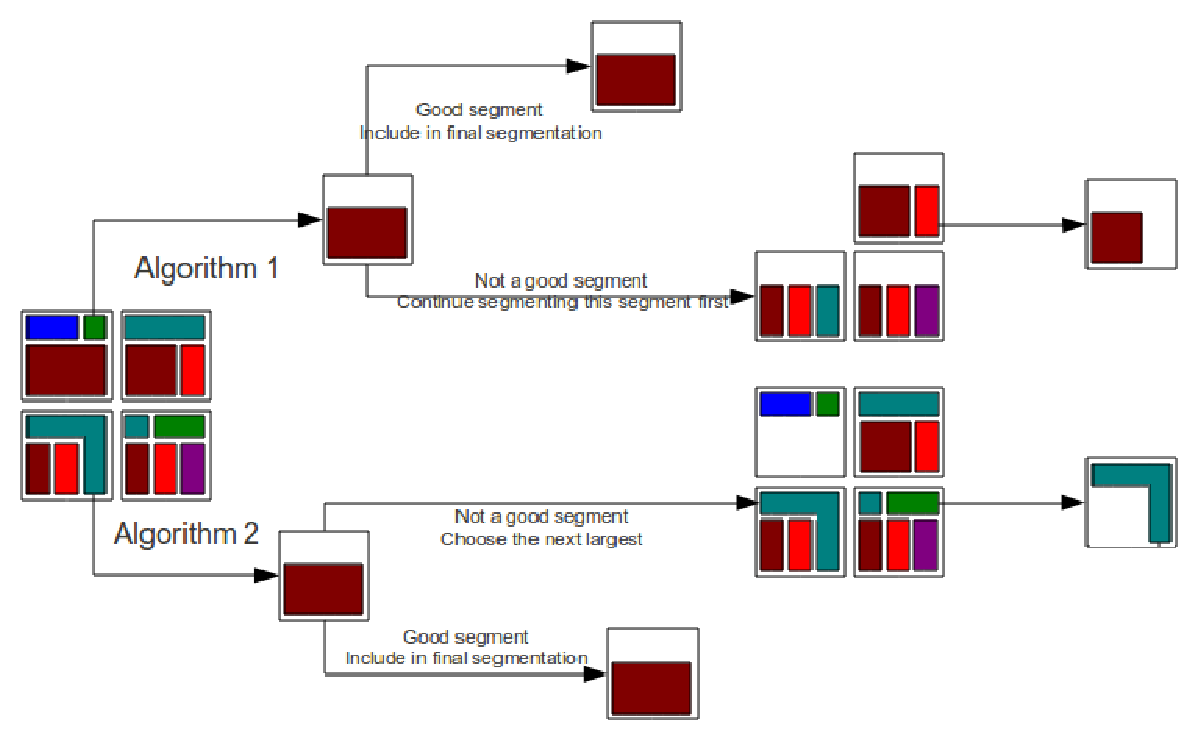
\includegraphics[scale =.8]{./Figures/mixsegs.eps}
\centering
\caption{2 Steps in mixing 4 different segmentations with the two algorithms
segments are represented by large colorful squares to better clarify the idea.}
\label{fig:mixsegsalgo}
\end{figure}

As shown in the pseudo-code in Algorithm \ref{alg:mixall1}, we take the largest
segment from all segmentations and try to check if this segment is a good
segment. If the segment is not good, we try to segment it recursively using the
other segmentations. Afterwards, we segment the remaining part of the image
similarly. However, in Algorithm \ref{alg:mixall2},
we always favor large segments on the image level. In other words, if the
largest segment isn't a good segment,
we choose the second largest segment in the whole image and check if it's a good
segment. In figure \ref{fig:mixsegsalgo}, we also provide a graphical
explanation for the two mixing techniques.

The only part remaining now is how to determine whether the segment is good or
not. To do that, we had to find a way for good segments evaluation.
First, we investigated in the the possibility of assuming that the color of each
region should follow a
normal distribution. In figure \ref{fig:colorhists}, we show a region of the
image and the colour histogram
of the three channels. The check for normality didn't work the way we expected.
Even while smoothing
the histograms, still sometimes the normality test fails for a perfectly
``good'' region. Figure \ref{fig:histn} shows an example that good regions
may not follow a normal distribution on real images.

Second, we tried the unimodality test. We checked if the distribution of the
histogram of each channel
follow unimodal function. We tried Dip test for unimodality by
\cite{dip-unimodality}. The resulting
segments were slightly better than those provided by the normality test but are
still too much. Figure \ref{fig:histn} also shows an example for failure of
unimodality test to determine a really good segment.

Third, we tried using the outliers detection method which will be described
later. Fourth we tried
the RAD method which gives our state of the art results. Finally, we tried the
alternative segmentation
technique. We'll describe the previous three techniques in the next sections.
\begin{figure}[!t]
\centering
\subfigure[] {
    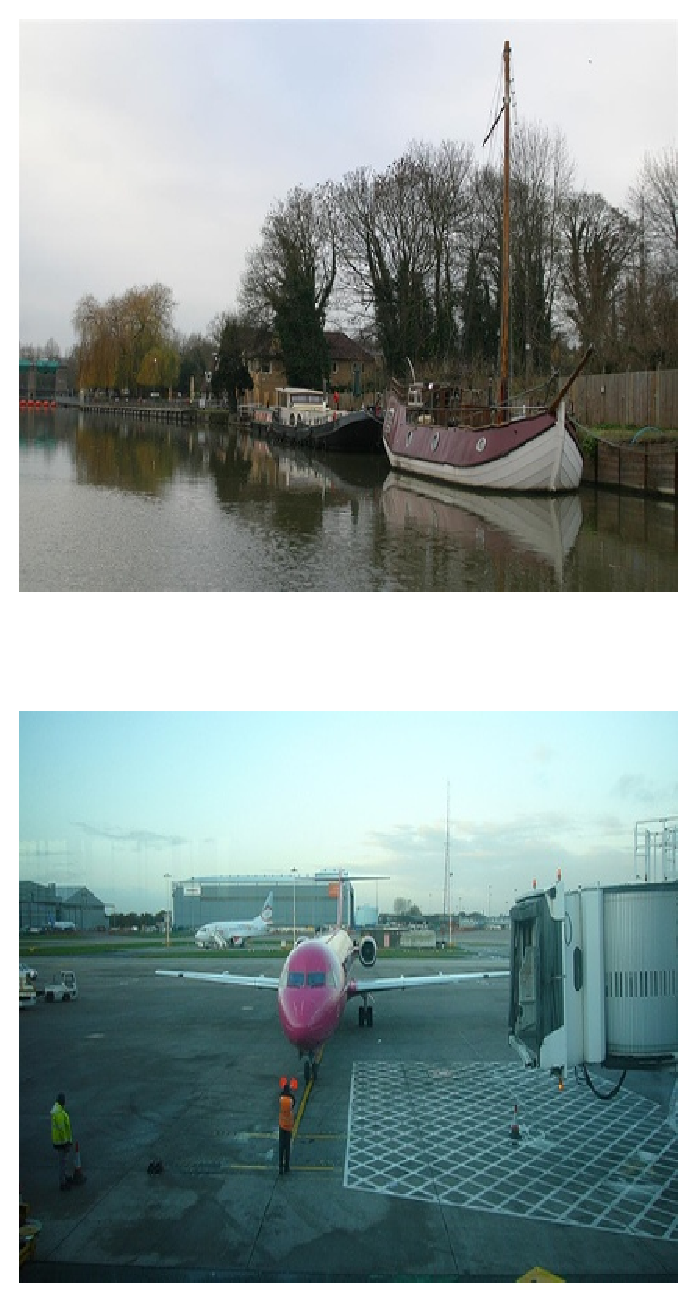
\includegraphics[width=150pt,height=290pt]{./Figures/orgnormality2.eps}
    \label{fig:orgn}
}
\subfigure[] {
    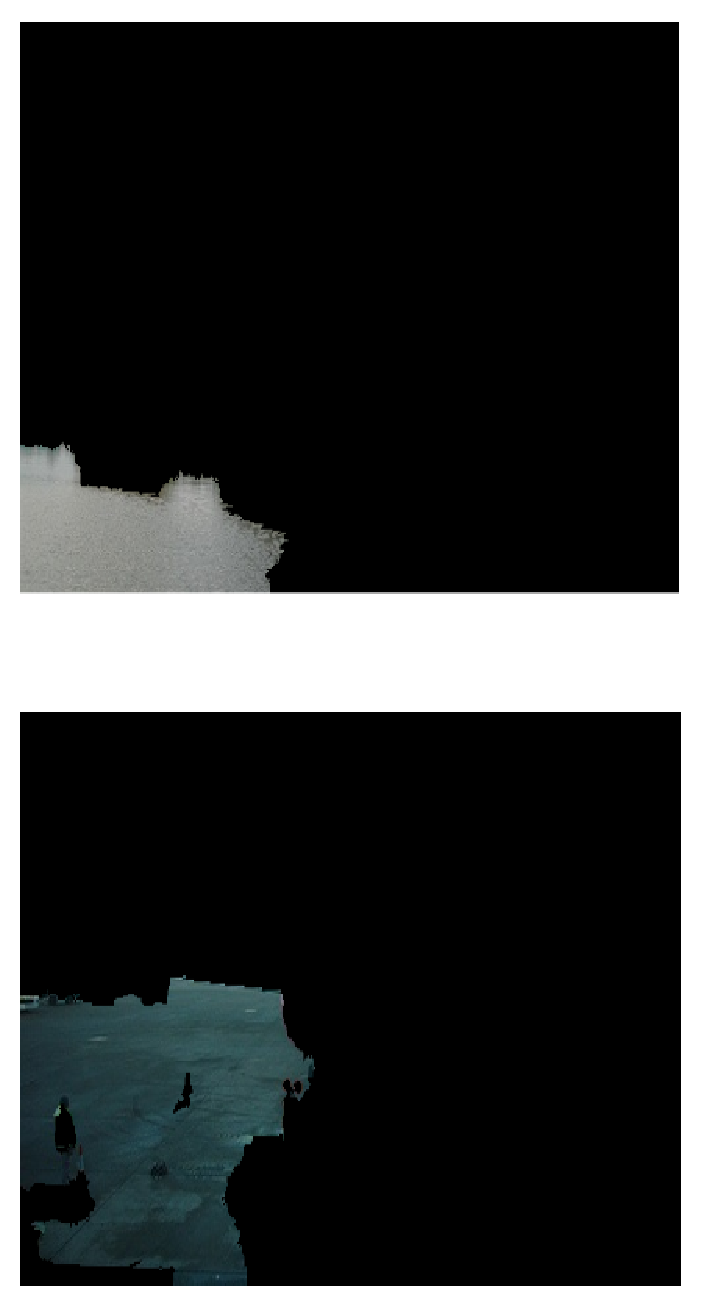
\includegraphics[width=150pt,height=290pt]{./Figures/segnormality2.eps}
    \label{fig:segn}
}
\subfigure[] {
    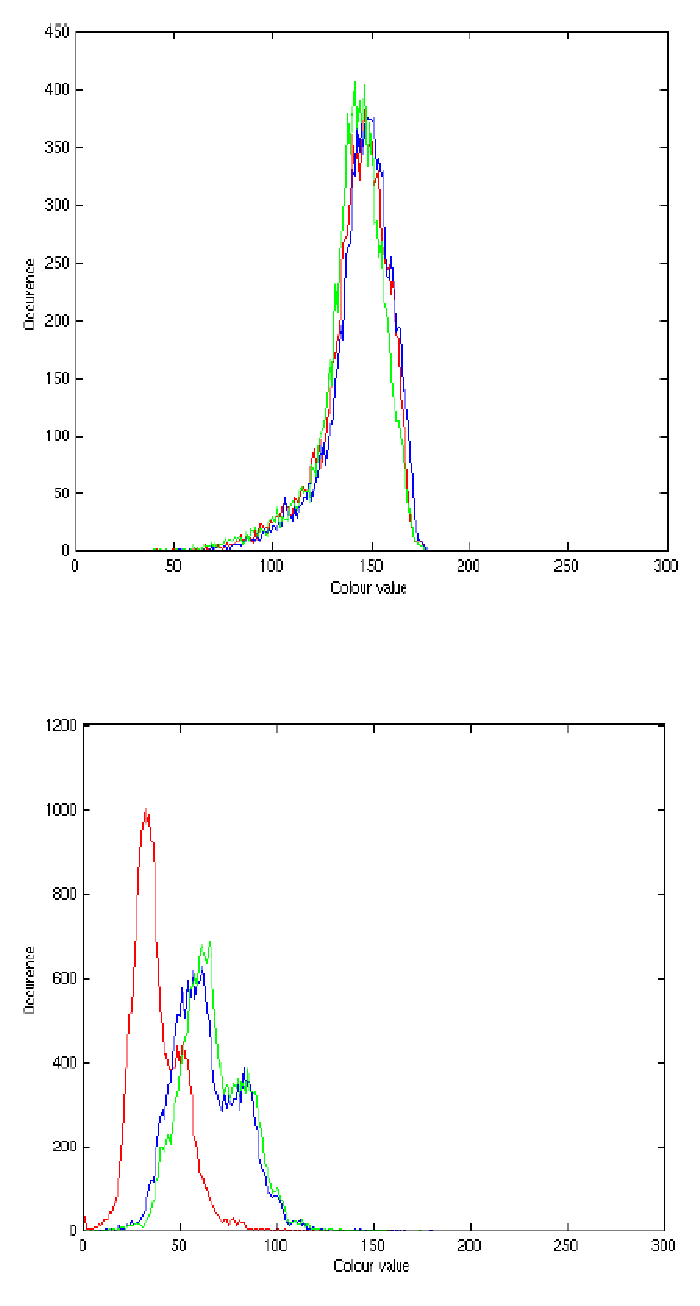
\includegraphics[width=150pt,height=290pt]{./Figures/histnormality2.eps}
    \label{fig:histn}
}
\caption{(a) Original images (b) Current largest segments (c) Histograms from
every
channel. As we can see the first image can be approximated into a normal distribution
or a unimodal distribution while the second one fails in that test.}
\label{fig:colorhists}
\end{figure}

\subsubsection{Good Segments evaluation using outliers finding}

As defined by \cite{grubbs-1969}, ``An outlying observation, or outlier, is one
that appears to deviate markedly from other members of the sample in which it
occurs.'' We consider a segment good if the number of outliers inside the
segment is less than a certain value. We did a series of experiments to
empirically determine the best value for the tolerance of outliers inside the
segment. We finally decided that a segment is considered good if the number of
outliers lying inside is less than 2\% of the number of pixels in the segment.

We use the Z-Test to find the outliers of a certain segment. The Z-Test
indicates that the point is considered an outlier if it satisfies the following
formula:

\[
\frac{|X - \mu|}{\sigma} > 3,
\]

where X is a label for each point of the image, $\mu$ is the mean of the color values
of each segment and $\sigma$ is the standard deviation of these colors.

Figure \ref{fig:mix_out} shows the results from mixing the different
segmentations using outlier finding. It also shows the number of generated
segments which is quite large due to our highly restricting criteria for
segments evaluation.

Although outliers detection worked well in detecting the segments in Figure
\ref{fig:segn}, they didn't work on detecting the segment in Figure
\ref{fig:outlier_not_seg}. In this segment the variations in colour are
really large and the different colours are not outliers in this case. Consequently,
we had to find another evaluation method that works well in the presence of shadows
and illuminations. This method is the RAD evaluation method explained in the next
section.

\begin{figure}[!t]
\centering
\subfigure[] {
    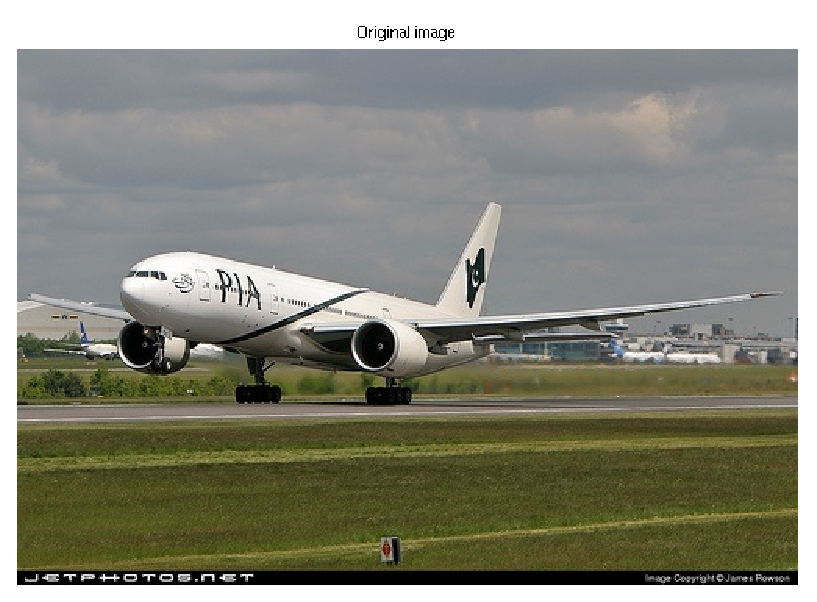
\includegraphics[width=150pt,height=120pt]{./Figures/ORG.eps}
    \label{fig:org}
}\\
\subfigure[] {
    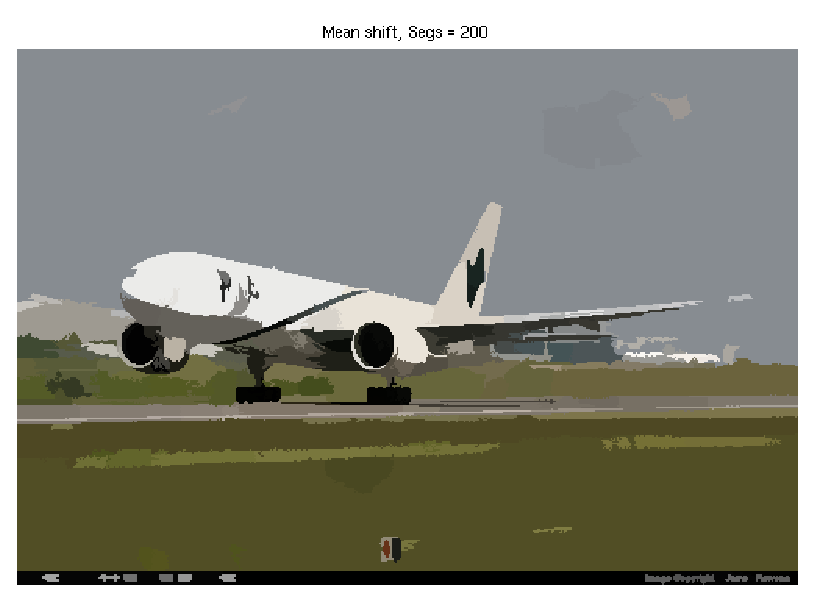
\includegraphics[width=150pt,height=120pt]{./Figures/MS.eps}
    \label{fig:ms}
}
\subfigure[] {
    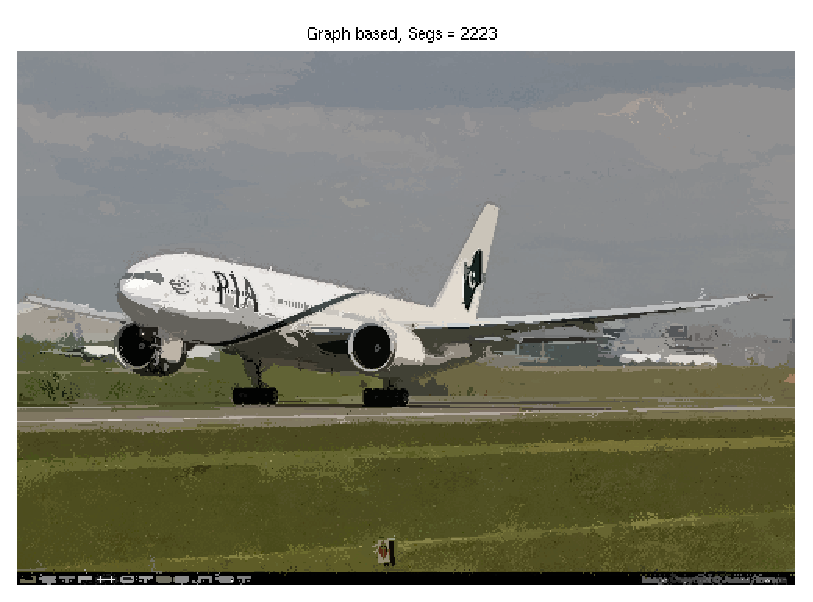
\includegraphics[width=150pt,height=120pt]{./Figures/GB.eps}
    \label{fig:gb}
}
\subfigure[] {
    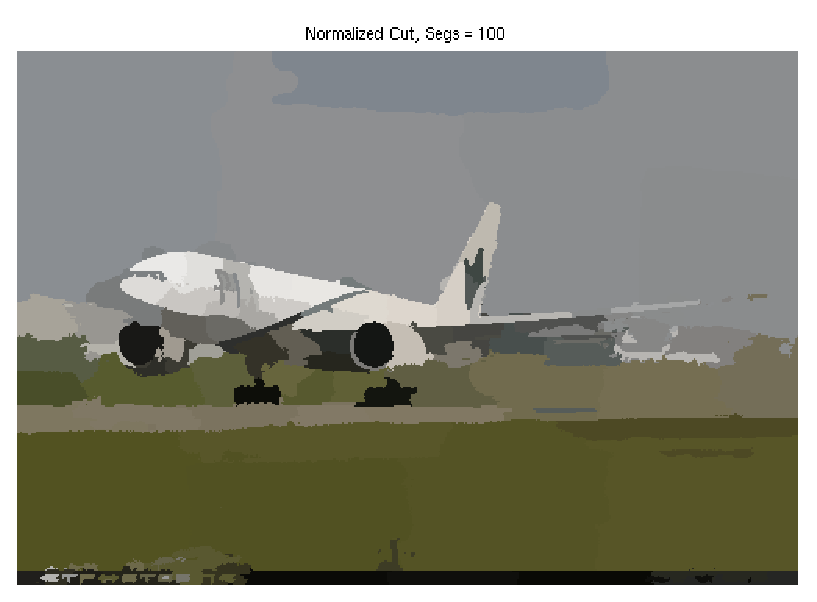
\includegraphics[width=150pt,height=120pt]{./Figures/NC.eps}
    \label{fig:nc}
}\\
\subfigure[] {
    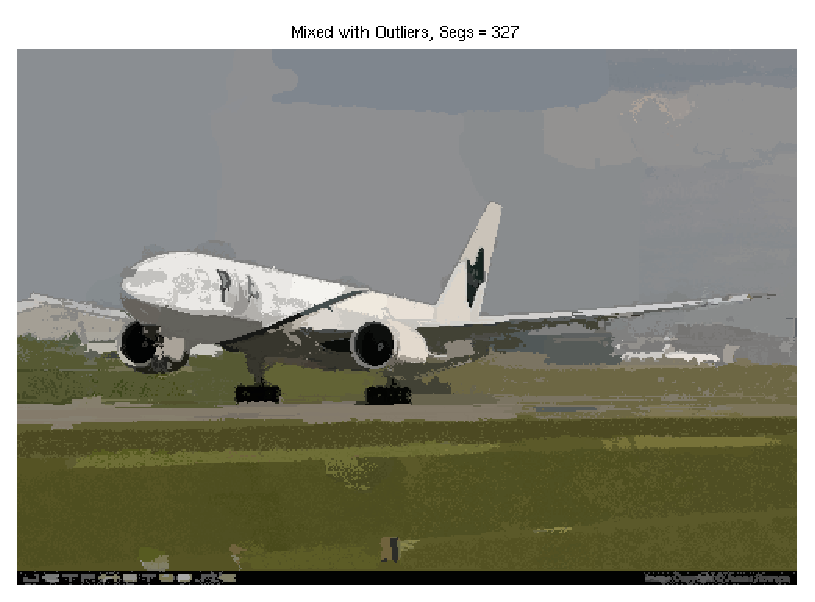
\includegraphics[width=150pt,height=120pt]{./Figures/Mixed_Outliers.eps}
    \label{fig:mix_out}
}
\subfigure[] {
    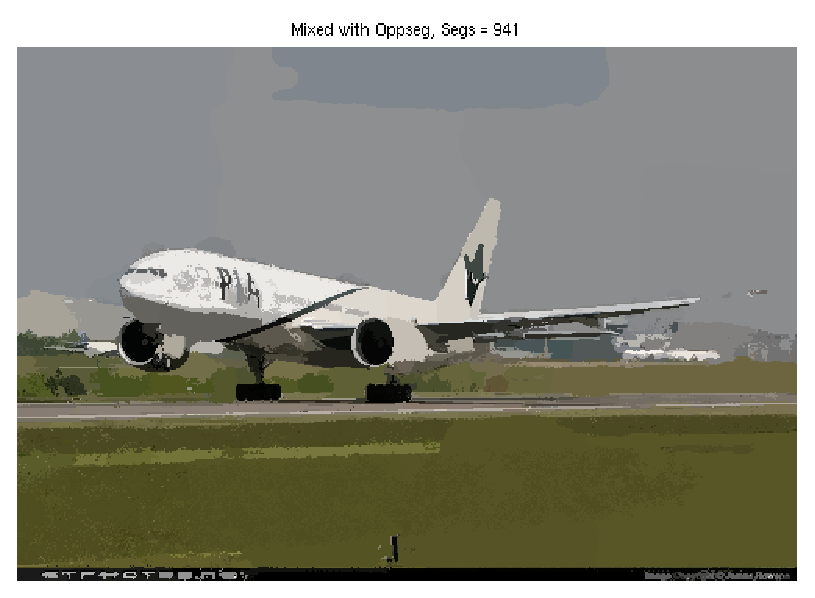
\includegraphics[width=150pt,height=120pt]{./Figures/Mixed_Opp.eps}
    \label{fig:mix_opp}
}
\subfigure[] {
    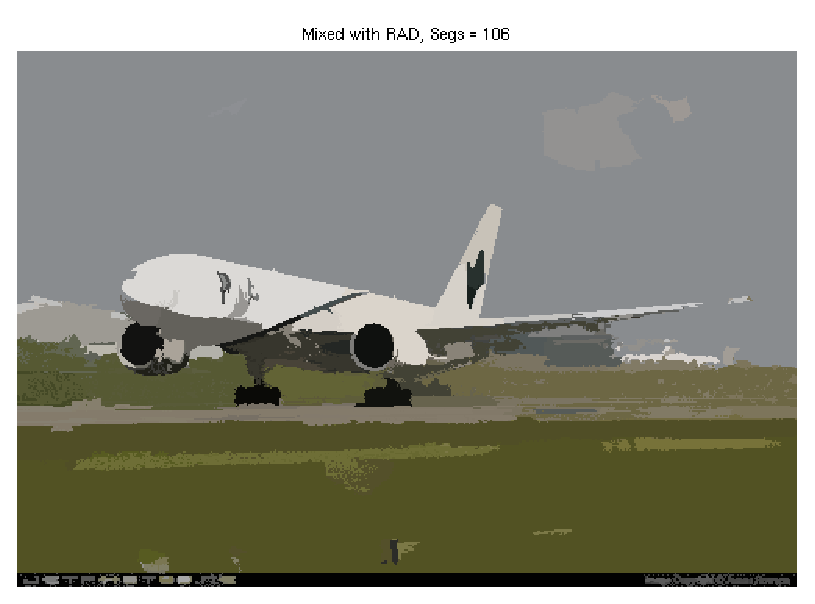
\includegraphics[width=150pt,height=120pt]{./Figures/Mixed_RAD.eps}
    \label{fig:mix_rad}
}
\caption{(a) Original image (b) Image segmented using mean shift. Number of
segments = 200 (c) Image segmented using Graph Based technique by
\cite{Felzenszwalb04efficientgraph-based}. Number of segments = 2223 (d) Image
segmented using normalized cut. Number of segments = 100 (e) Image segmented
using mixing and evaluation by finding outliers. Number of segments = 327
(f) Image segmented using mixing and evaluation by Alternate segmentation.
Number of segments = 941 (g) Image segmented using mixing and evaluation
by RAD. Number of segments = 106}
\label{fig:mix_allsegs}
\end{figure}

\begin{figure}[!t]
\centering
\subfigure[] {
    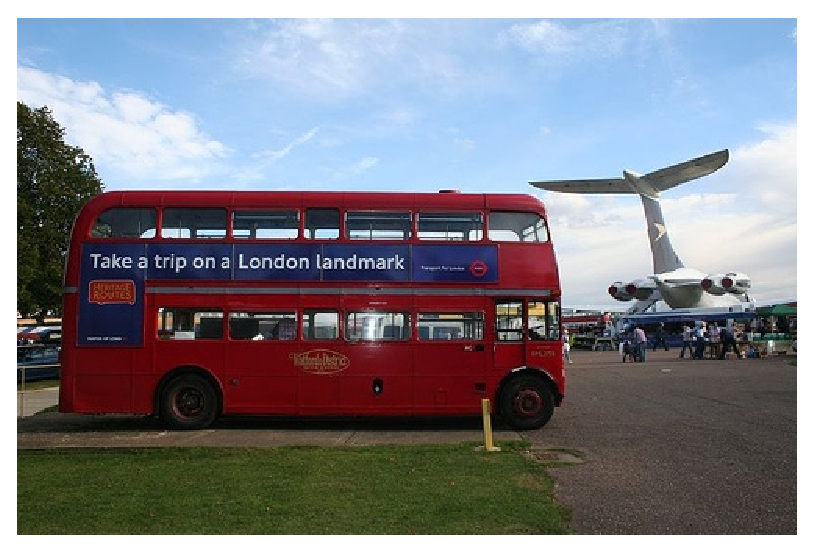
\includegraphics[width=150pt,height=120pt]{./Figures/outlier_not_org.eps}
    \label{fig:outlier_not_org}
}
\subfigure[] {
    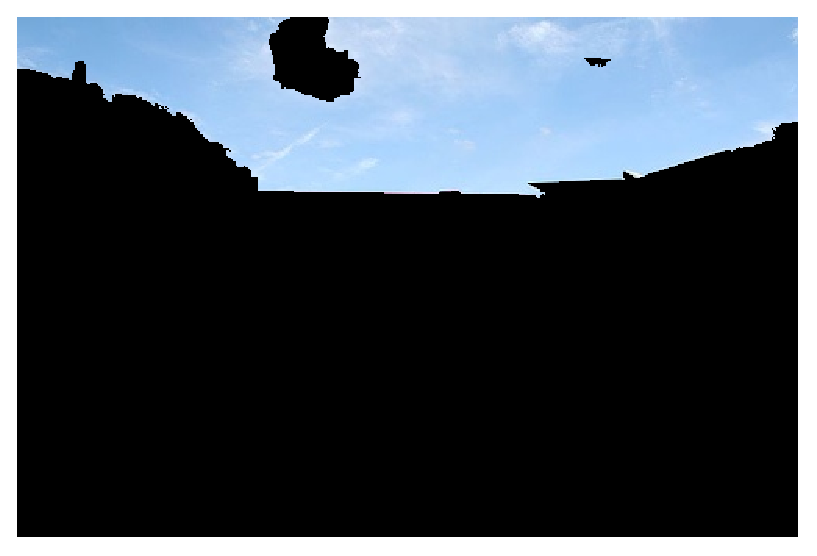
\includegraphics[width=150pt,height=120pt]{./Figures/outlier_not_seg.eps}
    \label{fig:outlier_not_seg}
}
\subfigure[] {
    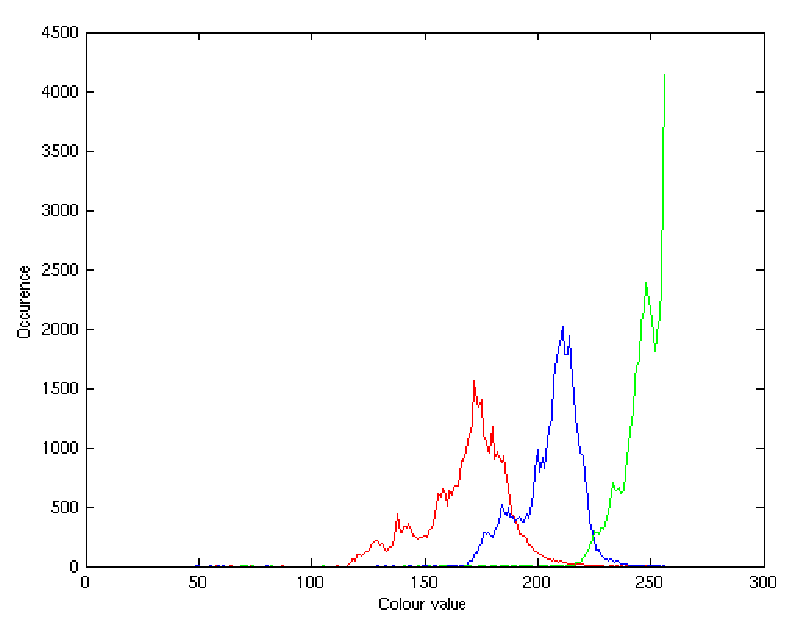
\includegraphics[width=150pt,height=120pt]{./Figures/outlier_not_hist.eps}
    \label{fig:outlier_not_hist}
}
\caption{(a) Original image (b) Current largest segment where outlier isn't working
(c) The image colour histogram for every channel }
\label{fig:outlier_not}
\end{figure}

\subsubsection{Good Segments evaluation using RAD}

We use the same method presented by \cite{1478239} for obtaining image
segmentations in the presence of shadows and highlights. This method is based on
the insight that the distributions formed by a single-colored object have a
physically determined shape in the colour histogram space. To capture
these ridges they proposed a new ridge based distribution analysis (RAD) to find
the set of ridges representative of the dominant colour.

We model the region ``segment'' as a set of dominant colours (DC). This DC is
described by a distribution in histogram-space. We assume that if this segment
contains only 1 DC then this segment is a ``good'' segment as this segment
contains only 1 semantic object.
Based on this technique, the evaluation method becomes very robust to shadows
and highlights and becomes closely related to the physical features of each
segment than the previous method.

To perform this evaluation we need to use the first step done by \cite{1478239}
in their segmentation technique which is extracting ridges as a representative
of a dominant structure (DS). Afterwards, we check if we have only one single
ridge in the image then we consider this segment as a good segment.

\paragraph{A Ridge based Distribution Analysis method}

In this section we will briefly explain the algorithm used by \cite{1478239} to
extract DCs from histogram space. They introduced a technique to find dominant
structures (DS) for a d-dimensional feature space. In our context here, a
dominant color is the dominant structure of the 3D chromatic histogram. We only
consider the segment good if it contains a single dominant colour.

First, we start by reviewing the dichromatic reflection model by \cite{136817}:

\begin{equation}
f(x) = m^{b}(x)c^{b} + m^{i}(x)c^{i},
\end{equation}

in which f = {R, G, B}, $c^{b}$ is the body reflectance, $c^{i}$ is the surface
reflectance, $m^{b}$ and $m^{i}$ are geometry dependant scalars representing the
magnitude of body and surface reflectance.

The two parts of the dichromatic reflectance model are clearly visible in the
histogram of figure \ref{fig:rpd}. First, due to the shading variations, the
distribution of the red pepper traces an elongated shape in histogram-space.
Second, the surface reflectance forms a branch which points in the direction of the reflected
illuminant. From the image, we can clearly condlude that the distribution of a
single DC doesn't really follow two straight lines as expected from the
dichromatic reflectance model due to the gamma, compressions, camera aberrations
or interreflections. Instead, they form a ridge-like structure in the histogram
space.

\begin{figure}[!t]
\centering
\subfigure[] {
    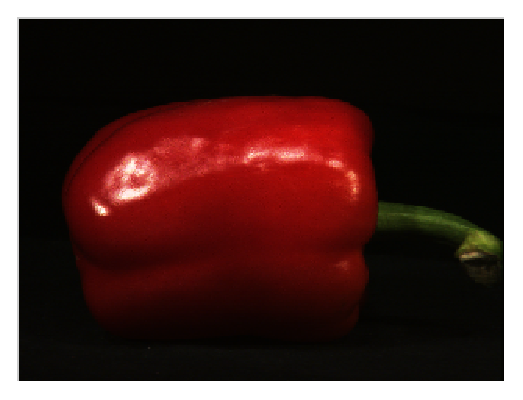
\includegraphics[width=90pt,height=70pt]{./Figures/red_pepper.eps}
    \label{fig:rp}
}
\subfigure[] {
    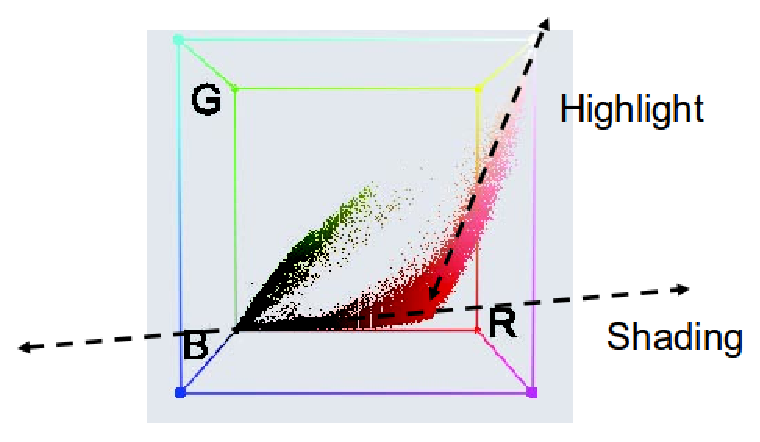
\includegraphics[width=120pt,height=70pt]{./Figures/red_pepper_dist.eps}
    \label{fig:rpd}
}
\subfigure[] {
    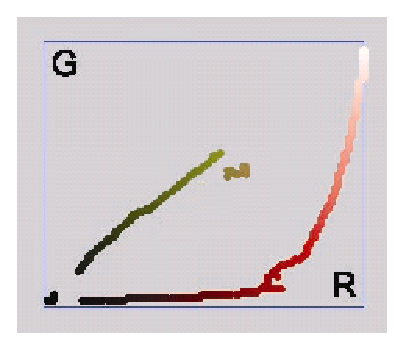
\includegraphics[width=90pt,height=70pt]{./Figures/red_pepper_ridges.eps}
    \label{fig:rpr}
}
\subfigure[] {
    
\includegraphics[width=90pt,height=70pt]{./Figures/red_pepper_seg.eps}
    \label{fig:rps}
}
\caption{(a) Original image (b) The image's histogram. The effects of shading
and highlights are clearly visible in the red colours of the histogram. (c)
Ridges found with RAD (d) Final segmented image. Image by \cite{1478239}}
\label{fig:pepper_rad}
\end{figure}

Another conclusion is what we can get from figure \ref{fig:horse_all}. Consider
figure \ref{fig:horsep} which contains a patch of the horse image. The 2D
Red-Green histogram of the patch is shown in figure \ref{fig:horseh} to see the
occurrences of the dichromatic combinations. It's clearly seen that the density
of the term $m^{b}$ varies significantly. The distribution is even broken into
two parts although they both belong to the same DC.

\begin{figure}[!t]
\centering
\subfigure[] {
    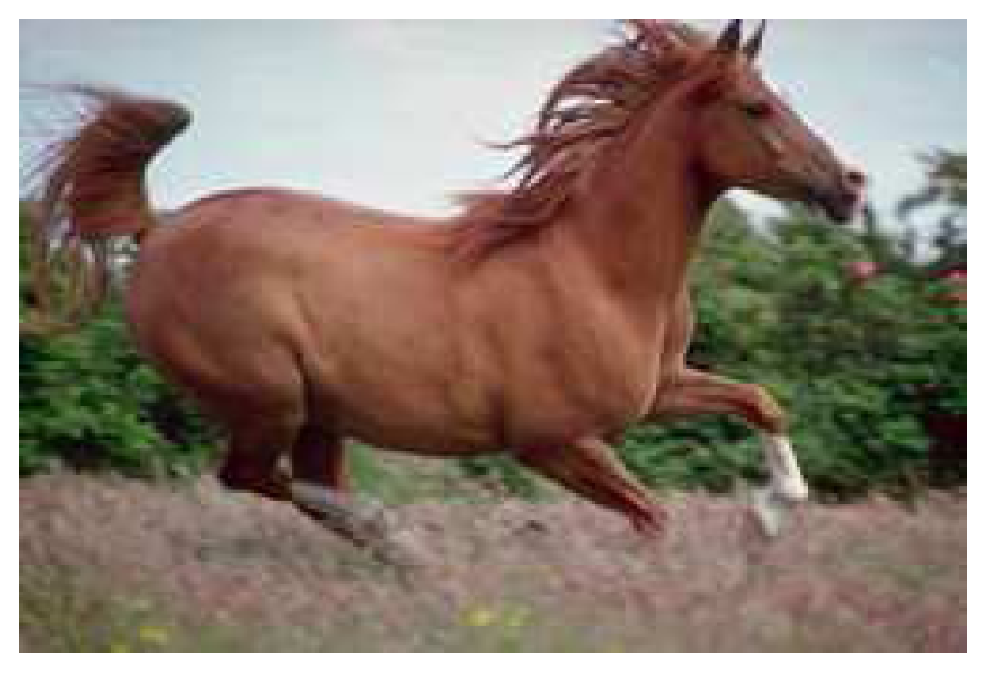
\includegraphics[width=120pt,height=80pt]{./Figures/horse.eps}
    \label{fig:horse}
}
\subfigure[] {
    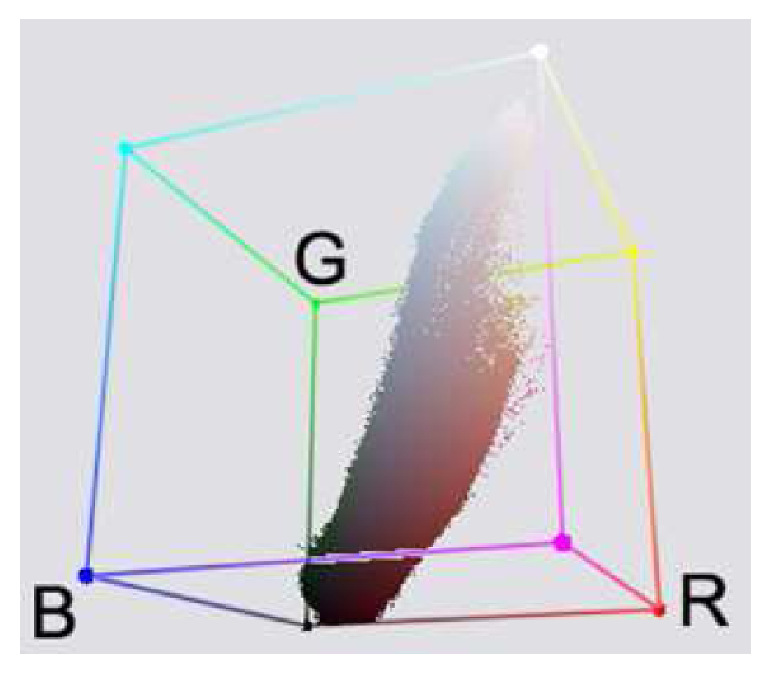
\includegraphics[width=80pt,height=80pt]{./Figures/horse_dist.eps}
    \label{fig:horsed}
}
\subfigure[] {
    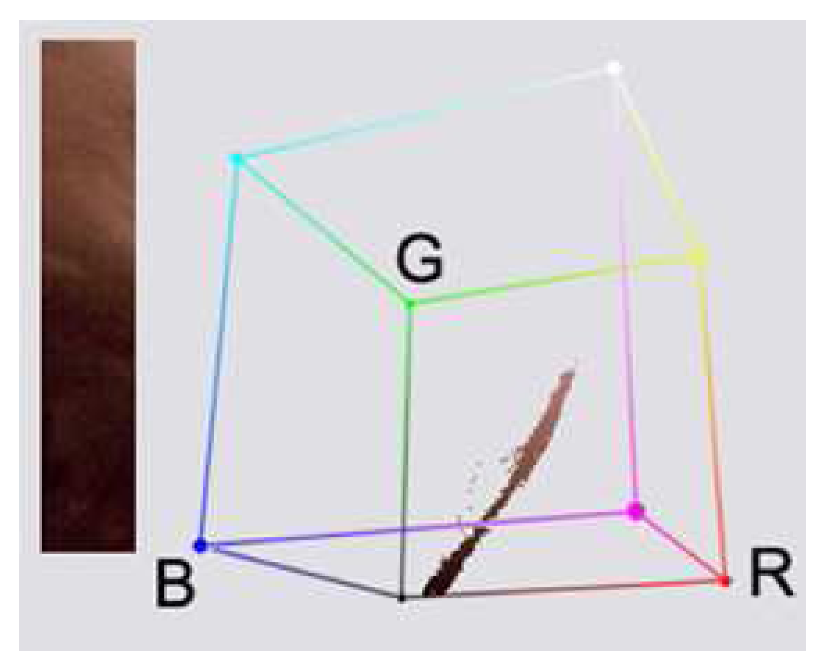
\includegraphics[width=80pt,height=80pt]{./Figures/horse_patch.eps}
    \label{fig:horsep}
}
\subfigure[] {
    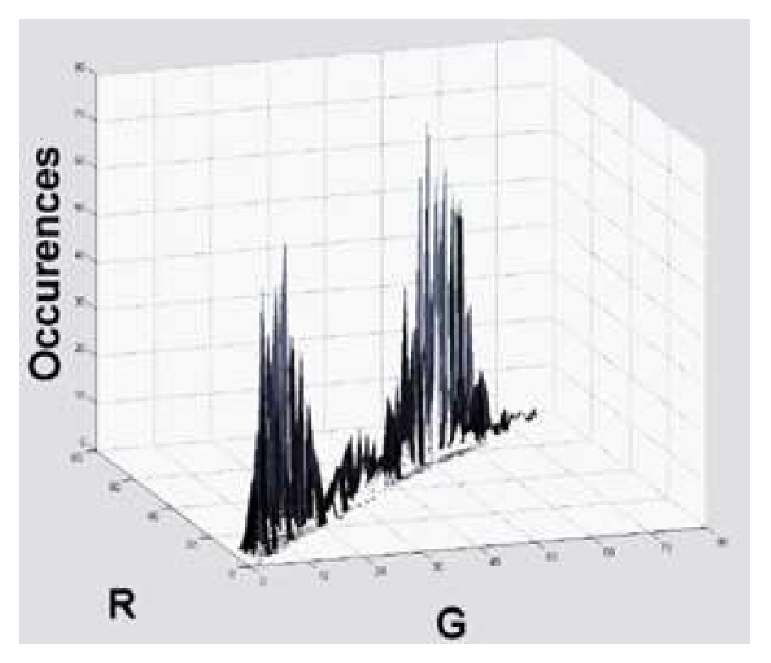
\includegraphics[width=90pt,height=80pt]{./Figures/horse_hist.eps}
    \label{fig:horseh}
}
\caption{(a) Original image (b) The image's RGB histogram. (c) A patch of a) and
it's RGB histogram (d) 2D histogram of c) to illustrate discontinuities on a DC.
Image by \cite{1478239}}
\label{fig:horse_all}
\end{figure}

From the previous two examples we conclude that we have two main shortcomings
from the dichromatic reflection model in describing what actually happens with
the real world images. The first one is how to deal with non-linearities and how
to get an approximation of the actual structure formed by the image's colour
histogram. The second, is dealing with the gaps in the colour histogram obained
within dominant structures of the same dominant colour.

To solve these problems, \cite{1478239} applied a multilocal creaseness
algorithm to overcome the gaps problem in the image's colour histogram.
Afterwards, they introduced a ridge extraction technique to avoid limitations of
linear assumption.

\subparagraph{Problem 1: Filling the gaps in the colour histogram}

In order to deal with the discontinuities in the image's colour histogram we
applied the MLSEC-ST operator introduced by \cite{crestes} to enhance ridge
points before the ridge detection step. This method is used due to its good
performance comnpared with other ridge detection methods on irregular and noisy
landscapes as explained by \cite{crestes}.

The structure tensor (ST) computes the dominant gradient orientation in a
neighbourhood of size proportional to $\sigma_{d}$. In other words, the operator
enhances the situations where either a big attraction (ridge) or a big repulsion
(valley) exist. Figure \ref{fig:crestes_exp} shows an example of applying the
MLSEC-ST operator on a 3D histogram.

\begin{figure}[!t]
\centering
\subfigure[] {
    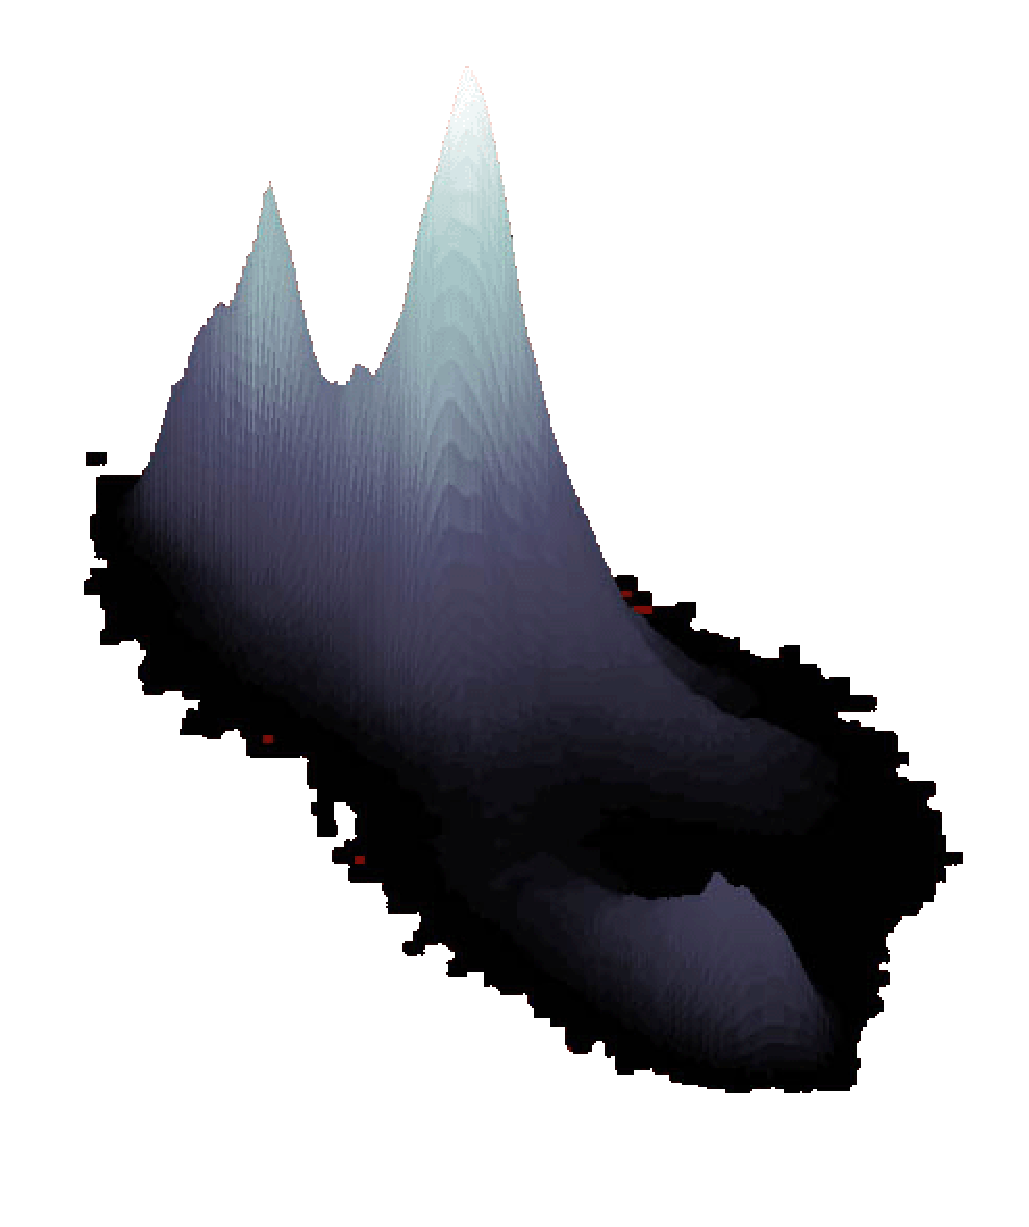
\includegraphics[width=90pt,height=90pt]{./Figures/hist.eps}
    \label{fig:hist}
}
\subfigure[] {
    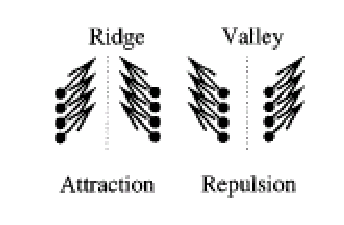
\includegraphics[width=120pt,height=90pt]{./Figures/ridgevalleyexpl.eps}
    \label{fig:rvexp}
}
\subfigure[] {
    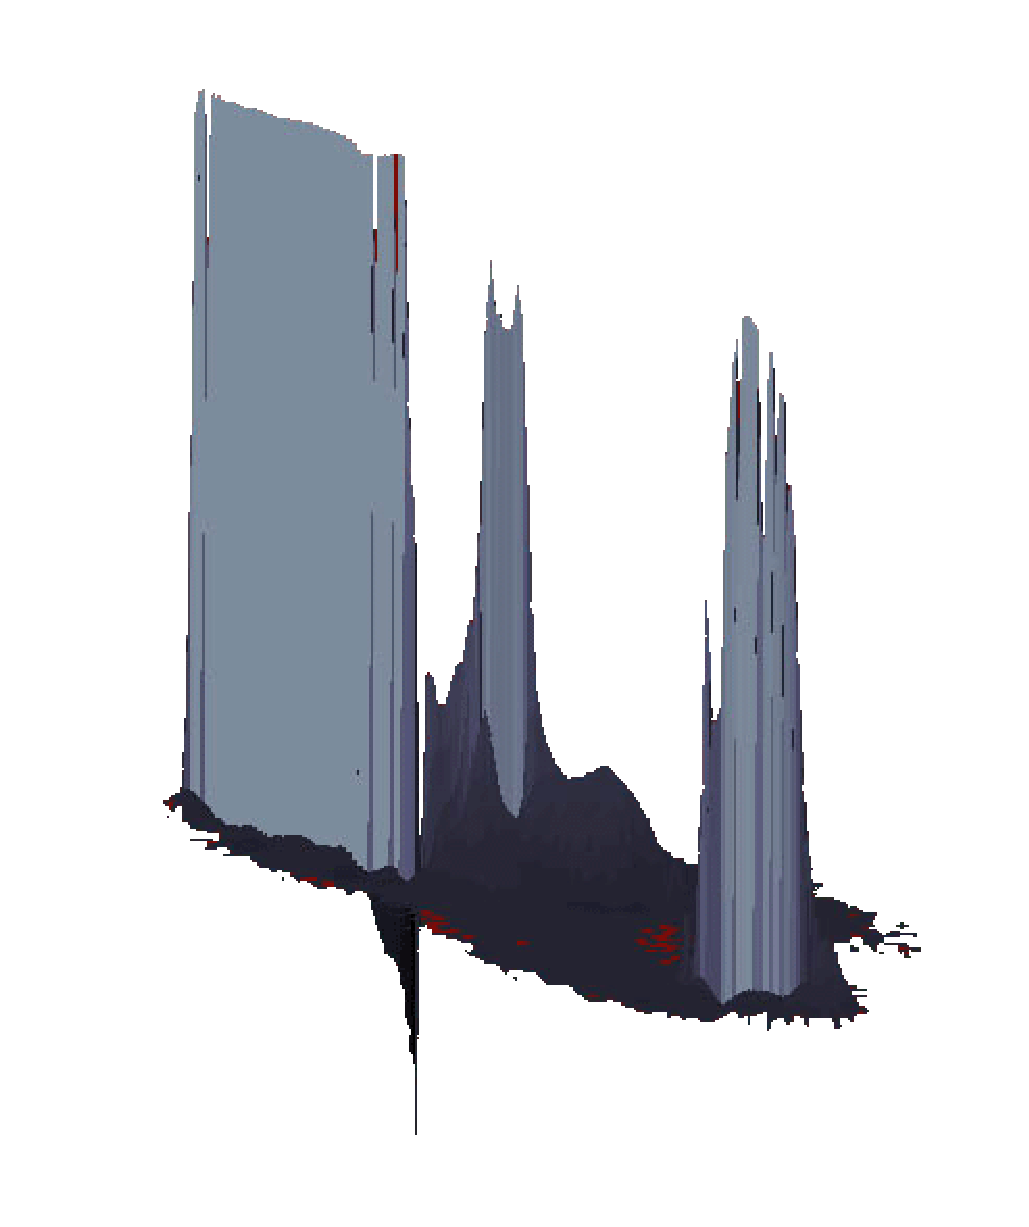
\includegraphics[width=90pt,height=90pt]{./Figures/crestes.eps}
    \label{fig:crestes}
}
\caption{(a) a 3D histogram (b) Points attracted to ridges and repulsed from
valleys. (c) MLSEC-ST applied to a). Image by \cite{1478239}}
\label{fig:crestes_exp}
\end{figure}

\subparagraph{Problem 2: Dealing with non-linearities}

To deal with non-linearities, we used the technique proposed by \cite{1478239}
for ridge detection. Their algorithm is briefly explained by algorithm
\ref{alg:ridgeext} and figure \ref{fig:ridges_exp}.

\begin{figure}[!t]
\centering
\subfigure[] {
    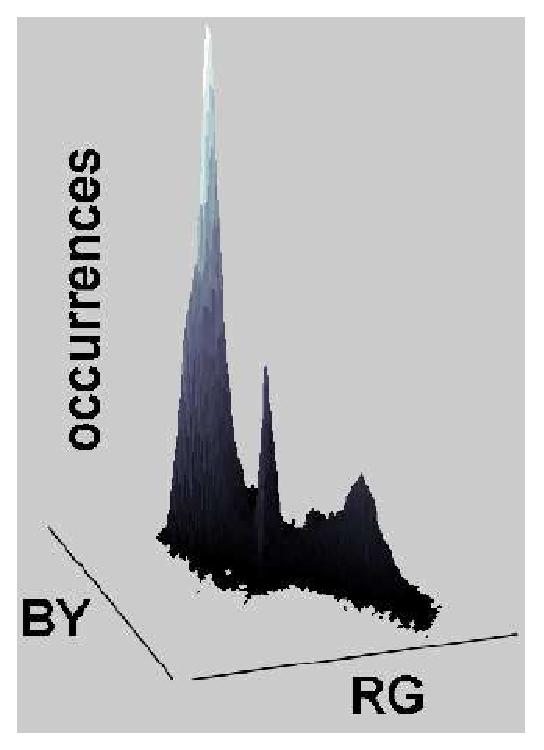
\includegraphics[width=90pt,height=90pt]{./Figures/a.eps}
    \label{fig:ahist}
}
\subfigure[] {
    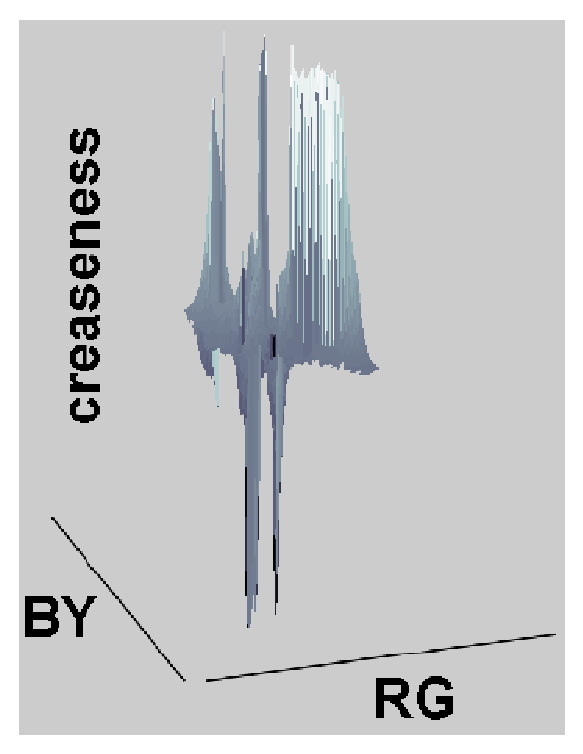
\includegraphics[width=90pt,height=90pt]{./Figures/b.eps}
    \label{fig:bcrestesa}
}
\subfigure[] {
    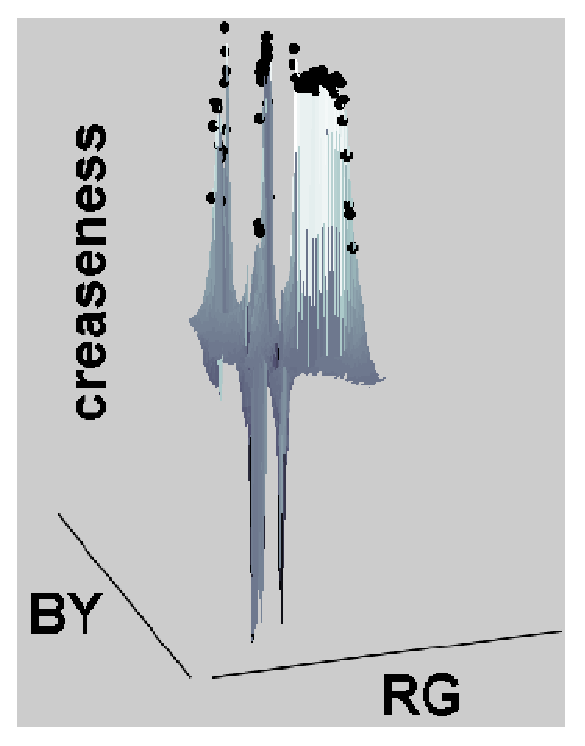
\includegraphics[width=90pt,height=90pt]{./Figures/c.eps}
    \label{fig:cridgesb}
}

\subfigure[] {
    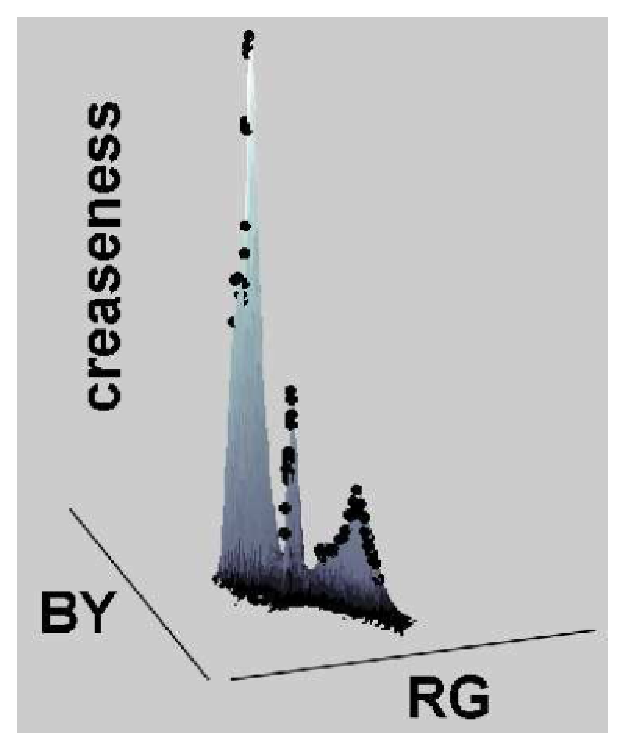
\includegraphics[width=90pt,height=90pt]{./Figures/d.eps}
    \label{fig:dridgesa}
}
\subfigure[] {
    \includegraphics[width=90pt,height=90pt]{./Figures/e.eps}
    \label{fig:etopd}
}
\subfigure[] {
    \includegraphics[width=90pt,height=90pt]{./Figures/f.eps}
    \label{fig:fdsa}
}
\caption{(a) Opponent red-green and blue-yellow histogram. (b) Creaseness
representation of a). (c) Ridges found in b). (d) Ridges fitted on the original
distribution. (e) Top view of d). (f) Dominant structures of a). Image from
\cite{1478239}}
\label{fig:ridges_exp}
\end{figure}

\begin{algorithm}
\caption{EXTRACT\_RIDGES}
\label{alg:ridgeext}
\begin{algorithmic}
\STATE Select a local maximum $m_{i}$
\STATE Add this local maximum to the list of ridge points. R = {$m_{i}$}
\IF {We reach a flat area}
\STATE stop;
\ELSE
\STATE repeat previous steps
\ENDIF
\end{algorithmic}
\end{algorithm}

After applying the ridge extraction algorithms. We check if there is more than one
ridge. In this case, clearly there is more than one dominant colour in this
region and, we discard the segment and look for an alternative segmentation of it.
Otherwise, we accept the segment is it is in our final segmentation.

In figure \ref{fig:mix_rad} we show one of our results from mixing segmentations
using segment evaluation with the described RAD criteria. Clearly, the number of
segments is reasonable. It is much less than those provided from the mixing and
evaluation using outliers detection method. Also the segments are meaningful as
they depend mainly on the image's colour histogram as an evaluator which gives
an important
clue about the distribution of colours in this segment.

It is worth mentioning here that despite being satisfactory while working with
shadows and highlights, RAD wasn't in our choices to perform the segmentation on
the PASCAL VOC 2007 dataset. RAD depends mainly on the MLSEC-ST operator. This
operator works much better with more colourful images that contain landscapes as
explained by \cite{crestes}. Consequently, RAD gives better segmentations for
some images but very bad segmentations for others. In figure \ref{fig:bad_seg_RAD}
we show an example of a really bad segmentation obtained by RAD on one of the images.
This behaviour is always repeated in the case that the illumination of the image
does not change considerably.

\begin{figure}[!t]
\centering
\subfigure[] {
    \includegraphics[scale =.4]{./Figures/bad_RAD_org.eps}
    \label{fig:bad_RAD_org}
}
\subfigure[] {
    \includegraphics[scale =.4]{./Figures/bad_RAD_RAD.eps}
    \label{fig:bad_RAD_RAD}
}
\caption{(a) Original image (b) Image segmented by RAD yielding an undesired
behaviour.}
\label{fig:bad_seg_RAD}
\end{figure}

\subsubsection{Good Segments evaluation using alternative segmentations}

Finally, we tried another method to evaluate the goodness of a segment which
is to try segmenting the same segment using another segmentation method which
differ in the way of extracting a segment.

Example: Mean-Shift segmentation mainly relies on the distribution of colours in
the segment, where graph-based segmentations mainly rely on the distribution of
edges in the segment.

This is mainly what we do for the evaluation of the segments using the
alternative segmentation method. In figure \ref{fig:mix_opp} we show the one if
the results obtained from mixing segmentations using the alternative segmentation
method.

\subsection{Describing and classifying regions from each segmentation}

Relying on the same framework by \cite{fulkerson09class}, we construct a bag
of features classifier which operates on the regions defined by the segments
obtained from each segmentation method. we use SIFT descriptors by for each pixel
in the image at a fixed scale and orientation.

We quantize the extracted descriptor using a K-means dictionary and we aggregate
them into one $l^1$ normalized histogram. For training the classifier, we assign
to each segment the  most frequent class label it contains. Afterwards, we train
a one-vs-rest support vector  machine (SVM) with an RBF-$\chi^2$ kernel on the
labeled histograms for each of the object categories.

The $\chi^2$ distance between histograms $h_i^0$ and $h^0$ is calculated using
the following formula:

\begin{equation}
d^2_{\chi^2}(h^0,h^0_i) = \sum_{m=1}^M{\frac{(h^0(m) - h^0_i(m))^2}{h^0(m) +
h^0_i(m)}}.
\end{equation}

From the previous equation it can be concluded that the larger the segment is, 
the more discriminative this distance will become. This is because the larger the
segment will be the more the information it will carry from the dictionary and the
more the variance will be in the final value of the distance which will lead
to better classification.

\subsection{Combining region classifications}

Similar to \cite{PSH08}, our approach towards combining multiple segmentations
revolve around
two main principles. The first is that pixels grouped together by every
segmentation should be
classified consistently. We use the same term used by \cite{PSH08} to describe
pixels that are
grouped together by each segmentation. We call them (IofRs) for Intersection of
Regions.

The second main principle is that to know an exact clue about these IofRs we
have to look at the whole segment obtained from each of the original segmentations.
In other words, the original  regions provide full support for extracting the
features of those IofRs.

To combine the IofRs by looking at whole segments, our input is the output of the SVM.
This output describes $P(c_r=k|r)$ where $c$ is the class label for region $r$
and $k\in{K}$ is a specific class label in the set of class labels $K$.

Now let $i$ be an IofR, $r_i^S$ is the region that contains $i$ in segmentation
$S$.

\[
\forall_{p\in{K}, q\in{K}}, P(c_i=p|I) > P(c_i=q|I) \propto
\frac{\sum_{m=1}^NP(c_i^{S_m} = p|r_i^{S_m},I) > P(c_i^{S_m} =
q|r_i^{S_m},I)}{N}
\]

Where $I$ is the original image and $N$ is the number of available segmentations
that we created.
This formula shows that an IofRs lies in class p with a higher probability than
a class q if in
several segmentations p lies in a better location than q. We also try to take
the position of p
and q into consideration. In other words, if p lies in the second location in
one of the segmentations
and on the first location on another segmentation, it's better than q if q lies
in the first location
in the first segmentation and the tenth location in the later one.

In figure \ref{fig:votation} we show a graphical explanation of our technique.
Also a pseudo code is
shown in algorithm \ref{alg:votation}.
\begin{algorithm}
\caption{class\_label = get\_class\_label(iofr, seg\_confs)}
\label{alg:votation}
\begin{algorithmic}
\STATE final\_confidences = zeros(classes\_count);
\FORALL {confidence segconf in seg\_confs}
\STATE [vals, indices] = sort(segconf);
\STATE final\_confidences(indices) += 1/indices;
\ENDFOR
\STATE [val, class\_label] = max(final\_confidences);
\RETURN class\_label;
\end{algorithmic}
\end{algorithm}

\begin{figure}
\includegraphics[scale =.4]{./Figures/votation.eps}
\centering
\caption{Voting scheme illustrated}
\label{fig:votation}
\end{figure}

\subsection{Refining results with a CRF}

This is the final step of our framework. In order to recover more precise boundaries
and reduce the effects of misclassifications inside the image, we finally refined
our results with a conditional random field.

In our framework, we didn't focus on enhancing the way of introducing the concept
of CRF. Instead, we used the same technique explained by \cite{fulkerson09class}.
We assumed the final segmentation $G(IofR, E)$ is an adjacency graph.
$P(c|G;w)$ is the conditional probability of the set of class label assignments c
where w is a weight.

\begin{equation}
-log(P(c|G;w)) = \sum_{IofR_i\in{S}}{\psi(c_i|IofR_i)} + \omega{\sum_{(IofR_i, IofR_j)\in{E}}{\phi(c_i,c_j|IofR_i,IofR_j)}}.
\end{equation}

Our unary potentials $\psi$ are obtained from probability outputs provided
by our SVM for each segment:

\[
\psi(c_i,s_i) = -log(P(c_i|s_i)),
\]

and our pairwise edge potentials $\phi$ are obtained using the following formula:

\[
\phi(c_i,c_j|s_i,s_j) = (\frac{L(s_i,s_j)}{1 + \parallel{s_i} - s_j\parallel})[c_i\neq{c_j}],
\]

where $\parallel{s_i} - s_j\parallel$ is the norm of the colour difference
between the two neighboring segments in the LUV colourspace. $L(s_i,s_j)$
is the shared boundary length between segments $s_i$ and $s_j$ and acts as
a regularizing term discouraging small regions. In figure \ref{fig:crf} we show an image
before and after applying the CRF operator in order to better clarify the idea.

\begin{figure}[!t]
\centering
\subfigure[] {
    \includegraphics[width=150pt,height=120pt]{./Figures/orgFigCRF.eps}
}
\subfigure[] {
    \includegraphics[width=150pt,height=120pt]{./Figures/befCRF.eps}
}
\subfigure[] {
    \includegraphics[width=150pt,height=120pt]{./Figures/aftCRF.eps}
}
\caption{(a) Original image (b) Segmented image before applying the CRF
operator. (c) Refined image after applying the CRF operator.}
\label{fig:crf}
\end{figure}

\section{Experiments}

Our results are divided into three main parts. The first part is an evaluation of
our new segmentation technique which is constructed from combining other segmentations
in a bottom-up fashion. We provide the results from using this method solely. In the
second part, we evaluated our votation technique applied only on the old
segmentations that we constructed. Finally, we add our new segmentation along
with the others and use the
votation scheme to get our final state of the art results.

We used VLBlocks by \cite{fulkerson09class} in our experiments. We added the
extra modules for mixing segmentations in various ways.

Figure \ref{fig:qual_res} shows some of the qualitative results resulting from
our framework.

\begin{figure}[!t]
\centering
\subfigure[] {
    \includegraphics[width=150pt,height=120pt]{./Figures/forg1.eps}
}
\subfigure[] {
    \includegraphics[width=150pt,height=120pt]{./Figures/gbqex.eps}
}\\
\subfigure[] {
    \includegraphics[width=150pt,height=120pt]{./Figures/ncqex.eps}
}
\subfigure[] {
    \includegraphics[width=150pt,height=120pt]{./Figures/msqex.eps}
}
\subfigure[] {
    \includegraphics[width=150pt,height=120pt]{./Figures/vcrfqex.eps}
}
\caption{(a) Original image (b) Final image segmented resulting from
our framework by applying the votation technique on the other segmentations.
(c) Image segmented by normalized cut then classified. (d) Image segmented
by mean shift then classified. (e) Image segmented by Graph-Based techniques
then classified.}
\label{fig:qual_res}
\end{figure}

\subsection{Experimental setup}

In this section we explain the different parameters we used to perform our
experiments.

We evaluated our method on one a standard, difficult data set: the
PASCAL VOC 2007 segmentation competition dataset. This dataset contains
multiple object classes with extreme variation in deformation, scale,
illumination, pose and occlusion. While the challenge specifies that the
detection challenge training data may also be used, we use only the 422 fully
segmented images to train our core approach. The performance measure for this
dataset is the average pixel accuracy: for each category the number of correctly
classified pixels is divided by the ground truth pixels plus the number of
incorrectly classified pixels. We also show the total percentage of pixels
correctly classified.

We extracted SIFT descriptors at each pixel using the quick SIFT technique in
the VLFeat framework by \cite{vedaldi08vlfeat}. The patch size for the SIFT
descriptors is 12 pixels. We quantize our descriptors into a K-means dictionary
learned using the training data. We chose $K = 400$ for all of the performed
experiments. \cite{fulkerson09class} stated in their experiments that changing
the value of $K$ still yields almost the same results. We didn't try to change K
but we used the same framework and we assumed their statements to be true.

Histograms with varying $N$ are extracted as described in section 3. For training,
labels are assigned to training segments coming from each segmentation by the
majority of class votes that we get from our training ground truth. We randomly
select an equal number of training histograms from each category as the training
data for our SVM.

We learn a one versus rest SVM model for each class with an RBF-$\chi^2$. We
used the libSVM tool by \cite{libsvm}. Finally, we refined our final labelled
results with a CRF model as described in section 4.5.

\subsection{Generating multiple segmentations}

In this section we will explain the different segmentations that we generated to
help us in the mixing process. We generated three types of segmentations,
Mean-shift segmentation by \cite{Comaniciu02meanshift}, Graph-based segmentation
by \cite{Felzenszwalb04efficientgraph-based} and normalized cut segmentation by
\cite{Shi_2000_3808}.

For the mean-shift segmentation we used the EDISON wrapper by
\cite{Christoudias02synergismin}. It is available online and has a good
performance. This code requires the following parameters: hs, indicating the
spatial bandwith for mean shift analysis, $hr$, indicating the range bandwidth
for mean shift analysis and $M$ which is the minimum size of final output regions.
For our experiments we used $hs = 11$, $hr = 8$ and $M = 40$.

For the efficient Graph-Based image segmentaton we used the code by
\cite{Felzenszwalb04efficientgraph-based}. The GB segmentation has two versions,
the adjacent neighborhood based and the $k$ nearest neighborhood based. We chose
the adjacent neighborhood based.
The following parameters are required: threshold, larger prefer larger segmented
area. minsize, the minimum size of segmentation component. $nRadius$, the radius
of neighbourhood of a pixel. We used the following values. $threshold = 0.5$,
$minsize = 50$, and $nRadius = 2$.

For the minimum cut we used the version explained by the work of \cite{1069213}.
They have publicly available source code on their website. The code only
requries the number of requested segments as its parameter. We chose the value of
100 to be the number of requsted segments each time.

We also generated an oversegmentation to obtain superpixels using quickshift by
\cite{vedaldi08quick}.These superpixels are controlled with the following three
parameters: $\lambda$, the tradeoff between color imprtance and spatial
importance, $\sigma$, the scale at which the density is estimated and $\tau$ the
maximum distance in the geature space between members of the same reguin. In our
experiments we used the folwing parameters, $\lambda = 0.5$, $\sigma = 2$ and,
$\tau = 8$.

In all our segmentations we chose our values after we applied several tries and
manually tuned the parameters values until we found the parameters that we
thought it better describes the segments and their boundaries. Figure
\ref{fig:seg_maps} shows the maps generated from segmentation of the
image in figure \ref{fig:org_map}.

\begin{figure}[!t]
\centering
\subfigure[] {
    \includegraphics[width=115pt,height=80pt]{./Figures/ORG3.eps}
    \label{fig:org_map}
}\\
\subfigure[] {
    \includegraphics[width=115pt,height=80pt]{./Figures/MSMap.eps}
    \label{fig:ms_map}
}
\subfigure[] {
    \includegraphics[width=115pt,height=80pt]{./Figures/GBMap.eps}
    \label{fig:gb_map}
}
\subfigure[] {
    \includegraphics[width=115pt,height=80pt]{./Figures/NCMap.eps}
    \label{fig:nc_map}
}
\subfigure[] {
    \includegraphics[width=115pt,height=80pt]{./Figures/SPMap.eps}
    \label{fig:sp_map}
}
\caption{(a) Original image (b) Image segmentation map using mean shift. (c)
Image segmentation map using Graph Based technique by
\cite{Felzenszwalb04efficientgraph-based}. (d) Image segmentation map using
normalized cut. (e) Image segmentation map with superpixels using quickshift.}
\label{fig:seg_maps}
\end{figure}

\subsection{Superpixels versus meaningful segments}

In this section we show how using superpixels alone always obtains worse
results than those obtained from meaningful segments. We show that even
when the segmentations give a greater number of segments, still, the performance
of the meaningful segments is higher than those obtained by the superpixels.

\begin{table}
\centering
\begin{tabular}{|@{ }c@{ }||@{ }c@{ }|@{ }c@{ }|@{ }c@{ }|@{ }c@{ }|@{ }c@{ }|@{
}c@{ }|@{ }c@{ }|@{ }c@{ }|@{ }c@{ }|@{ }c@{ }|@{ }c@{ }|@{ }c@{ }|@{ }c@{ }|@{
}c@{ }|@{ }c@{ }|@{ }c@{ }|@{ }c@{ }|@{ }c@{ }|@{ }c@{ }|@{ }c@{ }|@{ }c@{ }||@{
}c@{ }|@{ }c@{ }|}\hline
& {\begin{sideways}Background\end{sideways}} &
{\begin{sideways}Aeroplane\end{sideways}} &
{\begin{sideways}Bicycle\end{sideways}} & {\begin{sideways}Bird\end{sideways}} &
{\begin{sideways}Boat\end{sideways}} & {\begin{sideways}Bottle\end{sideways}} &
{\begin{sideways}Bus\end{sideways}} & {\begin{sideways}Car\end{sideways}} &
{\begin{sideways}Cat\end{sideways}} & {\begin{sideways}Chair\end{sideways}} &
{\begin{sideways}Cow\end{sideways}} &
{\begin{sideways}Dinningtable\end{sideways}} &
{\begin{sideways}Dog\end{sideways}} & {\begin{sideways}Horse\end{sideways}} &
{\begin{sideways}Motorbike\end{sideways}} &
{\begin{sideways}Person\end{sideways}} &
{\begin{sideways}Pottedplant\end{sideways}} &
{\begin{sideways}Sheep\end{sideways}} & {\begin{sideways}Sofa\end{sideways}} &
{\begin{sideways}Train\end{sideways}} &
{\begin{sideways}TVmonitor\end{sideways}} & {\begin{sideways}Avg
Accuracy\end{sideways}} & {\begin{sideways}Avg segcount\end{sideways}}\\\hline
Superpixels    & 14 & 21 & 7  & 7  & 22 & 12 & 6  & 7  & 26 &\textbf{12} & 12 &
9  & 10 & 10 & 11 & 2
 & 7  & 18 & 35 & 13 & 22 & 13 & 1201\\
Mean-shift     & 16 &\textbf{25} & 12 & 8  & 16 & 7  & 15 & 15 &\textbf{52} & 10
& 9  & 12
 &\textbf{20} & 5  & 19 & 16 & 23 &\textbf{23} &\textbf{43} & 17 & 31 & 19 &
393\\
Graph-based    & 18 & 21 & 20 & 2  & 17 & 6  & 11 & 21 & 39 & 2  & 15 & 14 & 3 
& 5  & 37 & 8 
 &\textbf{33} & 5  & 7  & 29 & 15 & 16 &2444\\
Normalized cut &\textbf{37} & 17 &\textbf{25} &\textbf{24} &\textbf{27}
&\textbf{16} &\textbf{41}
 &\textbf{38} & 50 & 9  &\textbf{26} &\textbf{42} & 12 &\textbf{15} &\textbf{66}
&\textbf{30} & 10
 & 19 & 27 &\textbf{58} &\textbf{35} &\textbf{30} & \textbf{100}\\\hline
\end{tabular}
\label{tab:allsegs}
\caption{Comparison on the average accuracy for superpixels using quickshift by
\cite{vedaldi08quick}, mean-shift segmentation by \cite{Comaniciu02meanshift},
graph based segmentation by \cite{Felzenszwalb04efficientgraph-based} and
normalized cut segmentation by \cite{Shi_2000_3808}. We show the accuracy of
each class and the final average accuracy. We also show the number of segments
generated from each segmentation method.}
\end{table}

As we can see from table 1 and also from figure \ref{fig:sp_map}
that the superpixels alone don't carry any meaningful information. Therefore,
when using them in classification, the segments tend to have very low accuracy.
Even lower than the graph based which although contains more segments than those
provided by the superpixels, the segments are still more meaningful segments
which leads to higher accuracy achievement.

\subsection{Segments resulting from our new segmentation method}

In this section we show our results of combining multiple segmentations in a
bottom-up manner using each of the 3 previously explained techniques.
We compare our mixed segmentations using 2 metrics. The first one is the average
number of segments per segmentations. The second is the average accuracy
obtained from using each one of the segmentations.

In table 2 we show the values of the accuracy obtained by
different
segmentation mixing techniques for each class. In figure \ref{fig:mixed_bu} we
show the effect
of using segment neighbourhoods on the final value of the accuracy.

\begin{table}
\centering
\begin{tabular}{|@{ }c@{ }||@{ }c@{ }|@{ }c@{ }|@{ }c@{ }|@{ }c@{ }|@{ }c@{ }|@{
}c@{ }|@{ }c@{ }|@{ }c@{ }|@{ }c@{ }|@{ }c@{ }|@{ }c@{ }|@{ }c@{ }|@{ }c@{ }|@{
}c@{ }|@{ }c@{ }|@{ }c@{ }|@{ }c@{ }|@{ }c@{ }|@{ }c@{ }|@{ }c@{ }|@{ }c@{ }||@{
}c@{ }|@{ }c@{ }|}\hline
& {\begin{sideways}Background\end{sideways}}
& {\begin{sideways}Aeroplane\end{sideways}}
& {\begin{sideways}Bicycle\end{sideways}}
& {\begin{sideways}Bird\end{sideways}}
& {\begin{sideways}Boat\end{sideways}}
& {\begin{sideways}Bottle\end{sideways}}
& {\begin{sideways}Bus\end{sideways}}
& {\begin{sideways}Car\end{sideways}}
& {\begin{sideways}Cat\end{sideways}}
& {\begin{sideways}Chair\end{sideways}}
& {\begin{sideways}Cow\end{sideways}}
& {\begin{sideways}Dinningtable\end{sideways}}
& {\begin{sideways}Dog\end{sideways}}
& {\begin{sideways}Horse\end{sideways}}
& {\begin{sideways}Motorbike\end{sideways}}
& {\begin{sideways}Person\end{sideways}}
& {\begin{sideways}Pottedplant\end{sideways}}
& {\begin{sideways}Sheep\end{sideways}}
& {\begin{sideways}Sofa\end{sideways}}
& {\begin{sideways}Train\end{sideways}}
& {\begin{sideways}TVmonitor\end{sideways}}
& {\begin{sideways}Avg Accuracy\end{sideways}}
& {\begin{sideways}Avg segcount\end{sideways}}\\\hline
Outliers & 22 & 9  & 15 & 8  &\textbf{25} & 14 & 18 & 11& 43 &
11 & 13 &
 16 &\textbf{31} &\textbf{22} & 27 & 6  & 31 & 15 &\textbf{35} & 27 & 18 & 20 &
411\\
AltSeg & 10 &\textbf{33} & 17 & 3  & 2  &\textbf{22} & 14 & 9
& 44 &
 7  & 10 & 31 & 5  & 7  & 20 & 2  & 24 & 10 & 8  & 7  & 20 & 15 &1769\\
RAD  &\textbf{26} & 12 & 11 &\textbf{26} & 17 & 16
&\textbf{28} & 17
 &\textbf{53} &\textbf{14} & 14 & 40 & 28 & 21 & 50 & 20 &\textbf{50}
&\textbf{38} & 30 & 50 & 32 & 28 & 121\\\hline
Worst seg (Superpixels)   & 14 & 21 & 7  & 7  & 22 & 12 & 6  & 7 & 26 & 12 & 12
& 9  & 10
 & 10 & 11 & 2  & 7  & 18 & 35 & 13 & 22 & 13 & 1201\\
Best seg (Normalized cut) & 37 & 17 &\textbf{25} & 24 & 27 & 16 & 41
&\textbf{38}& 50 & 9
 &\textbf{26} &\textbf{42} & 12 & 15 &\textbf{66} &\textbf{30} & 10 & 19 & 27
&\textbf{58}
 &\textbf{35} &\textbf{30} & \textbf{100}\\\hline
\end{tabular}
\label{tab:mixed_segs}
\caption{Comparison on the average accuracy for mixing segmentations and
evaluating good segments using outliers detection, opposite segmentations
and RAD. We also include the worst segmentation (Superpixels) and the best
segmentation (Normalized cut) to include
them in the comparison. We show the accuracy of each class and the final average
accuracy. We also show the number of segments
generated from each segmentation mixing method.}
\end{table}
\begin{figure}
\includegraphics[scale =.65]{./Figures/neigh_mix.eps}
\centering
\caption{Effect of neighbourhood on the average accuracies}
\label{fig:mixed_bu}
\end{figure}

\subsection{Segments benchmarks from our new segmentation method}

We also performed a series of experiments on the Berkeley Segmentation Dataset and
Benchmark by \cite{MartinFTM01}. We evaluated our multiple segmentations with the
newly created segmentation based on RAD for evaluation. We measured 4 different
error measurements for evaluating our segmentations quality. However, the only
problem is that we didn't try several different parameters either for each of the
segmentation methods or for the RAD criteria for segments evaluation.

The 4 different error measures we tried are: First, the Probabilistic Rand Index
(PRI) by \cite{1099935} which counts the fraction of pairs of pixels whose labellings are
consistent between the computed segmentation and the ground truth, averaging across
multiple ground truth segmentations to account for scale variation in human perception.
The second error measure is the Variation of Information (VoI) by \cite{citeulike:3906686}.
It defines the distance between two segmentations as the average conditional entropy
of one segmentation given the other, and thus roughly measures the amount of randomness
in one segmentation which cannot be explained by the other.
The third is the Global Consistency Error (GCE) by \cite{MartinFTM01} that measures the
extent to which one segmentation can be viewed as a refinement of the other. Segmentations
which are related in this manner are considered to be consistent, since they could represent
the same natural image segmented at different scales.
The fourth measure is the Boundary Displacement Error (BDE) by \cite{649319}. It measures
the average displacement error of boundary pixels between two segmented images. Particularly,
it defines the error of one boundary pixel as the distance between the pixel and the
closest pixel in the other boundary image.

In table 3 we show the segmentations benchmark results. We see that our method improves
both the PRI and the VoI. Even though, we still need to repeat the experiments several times
with different parameters to be able to generalize our approach.

\begin{table}
\centering
\begin{tabular}
{|c||c|c|c|c|}
\hline
               & PRI             & VoI             & GCE             & BDE              \\\hline
Mean-Shift     & 0.7424          & 4.5293          & \textbf{0.0842} & \textbf{14.2716} \\\hline
Graph-Based    & 0.7082          & 5.1148          & 0.1150          & 17.2428          \\\hline
Normalized-cut & 0.7079          & 4.1370          & 0.1153          & 14.7337          \\\hline
Mix+RAD        & \textbf{0.7483} & \textbf{3.5364} & 0.1433          & 14.8047          \\\hline
\end{tabular}
\label{tab:seg_bench}
\caption{Segmentation benchmarks results for the Berkeley Segmentation Dataset and
Benchmark. 4 error measures were considered for 4 different segmentations.}
\end{table}

\subsection{Class segmentation results using the voting technique alone}

In this section, we describe the results obtained using the voting technique
for mixing several segmentations. We show how mixing segmentations using the
voting technique improves the overall average accuracy and also improves the
accuracy for many classes.

We tried to combine many different segmentations together and check for the results
using our voting technique and the technique explained by \cite{PSH08}.
We show the results in table 4.

\begin{table}
\centering
\begin{tabular}{|@{ }c@{ }||@{ }c@{ }|@{ }c@{ }|@{ }c@{ }|@{ }c@{ }|@{ }c@{ }|@{
}c@{ }|@{ }c@{ }|@{ }c@{ }|@{ }c@{ }|@{ }c@{ }|@{ }c@{ }|@{ }c@{ }|@{ }c@{ }|@{
}c@{ }|@{ }c@{ }|@{ }c@{ }|@{ }c@{ }|@{ }c@{ }|@{ }c@{ }|@{ }c@{ }|@{ }c@{ }||@{
}c@{ }|}\hline
& {\begin{sideways}Background\end{sideways}}
& {\begin{sideways}Aeroplane\end{sideways}}
& {\begin{sideways}Bicycle\end{sideways}}
& {\begin{sideways}Bird\end{sideways}}
& {\begin{sideways}Boat\end{sideways}}
& {\begin{sideways}Bottle\end{sideways}}
& {\begin{sideways}Bus\end{sideways}}
& {\begin{sideways}Car\end{sideways}}
& {\begin{sideways}Cat\end{sideways}}
& {\begin{sideways}Chair\end{sideways}}
& {\begin{sideways}Cow\end{sideways}}
& {\begin{sideways}Dinningtable\end{sideways}}
& {\begin{sideways}Dog\end{sideways}}
& {\begin{sideways}Horse\end{sideways}}
& {\begin{sideways}Motorbike\end{sideways}}
& {\begin{sideways}Person\end{sideways}}
& {\begin{sideways}Pottedplant\end{sideways}}
& {\begin{sideways}Sheep\end{sideways}}
& {\begin{sideways}Sofa\end{sideways}}
& {\begin{sideways}Train\end{sideways}}
& {\begin{sideways}TVmonitor\end{sideways}}
& {\begin{sideways}Avg Accuracy\end{sideways}}\\\hline
Votation Best Mix      &\textbf{48} & 20 & 21 &\textbf{16} & 10 &\textbf{30}
&\textbf{32} & 42 & 56 & 23 & 19 &\textbf{35} & 51 & 18 & 63 &\textbf{52}
&\textbf{28} & 20 & 29 & 40 & 34 &\textbf{33}\\
Votation Worst Mix     & 34 & 14 &\textbf{22} & 5  &\textbf{18} & 25 & 28 & 21 &
55 & 25 & 17 & 25 & 30 &\textbf{28} & 54 & 34 & 36 &\textbf{21} & 30 & 38 & 33 &
28\\\hline
\cite{PSH08} Best Mix  & 38 &\textbf{30} & 21 & 11 & 14 & 9  & 25 & 24
&\textbf{61} &\textbf{36} &\textbf{21} & 14 &\textbf{53} & 24 &\textbf{65}
&\textbf{52} & 27 & 15 &\textbf{31} &\textbf{42} &\textbf{42} & 31\\
\cite{PSH08} Worst Mix & 38 & 14 & 14 & 14 & 8  & 6  &\textbf{32} &\textbf{45} &
52 & 19 & 12 & 18 & 30 & 24 & 56 &\textbf{52} & 24 & 15 & 24 &\textbf{42} & 32 &
27\\\hline
\end{tabular}
\label{tab:mixed_comb}
\caption{Comparison on the average accuracy for mixing segmentations and
evaluating good segments by mixing segmentations using votations and
the technique proposed by \cite{PSH08}. In both cases the final best mix was
obtained by mixing all segmentations together and the worst mix was obtained
by only mixing the graph based segmentation with the mean shift.}
\end{table}

We compare our segments combination method with the one proposed by
\cite{PSH08}. We get better results in the final overall accuracy. Also notice
that
The best segmentation result is higher than the best accuracy achieved without
combining. Even the worst results are still good enough
and are way better than the results before mixing. The best results are obtained
on combining all segmentation results together while
the worst results are obtained when combining the mean shift with the graph
based segmentations. Note that still the results from combining those two
improved more than 10 percent over the results of the graph based alone and
almost 10 percent over the results of the mean shift alone.

\subsection{Class segmentation by using the voting technique with our new
segmentation method}

This is our final work until now. We combined all of the information that we
have had to get the best possible results. We used
the voting technique for mixing segmentations along with our newly created
segmentation. We also tried many possible permutations
for segments. We show our results in table 5.

\begin{table}
\centering
\begin{tabular}{|@{ }c@{ }||@{ }c@{ }|@{ }c@{ }|@{ }c@{ }|@{ }c@{ }|@{ }c@{ }|@{
}c@{ }|@{ }c@{ }|@{ }c@{ }|@{ }c@{ }|@{ }c@{ }|@{ }c@{ }|@{ }c@{ }|@{ }c@{ }|@{
}c@{ }|@{ }c@{ }|@{ }c@{ }|@{ }c@{ }|@{ }c@{ }|@{ }c@{ }|@{ }c@{ }|@{ }c@{ }||@{
}c@{ }|}\hline
& {\begin{sideways}Background\end{sideways}}
& {\begin{sideways}Aeroplane\end{sideways}}
& {\begin{sideways}Bicycle\end{sideways}}
& {\begin{sideways}Bird\end{sideways}}
& {\begin{sideways}Boat\end{sideways}}
& {\begin{sideways}Bottle\end{sideways}}
& {\begin{sideways}Bus\end{sideways}}
& {\begin{sideways}Car\end{sideways}}
& {\begin{sideways}Cat\end{sideways}}
& {\begin{sideways}Chair\end{sideways}}
& {\begin{sideways}Cow\end{sideways}}
& {\begin{sideways}Dinningtable\end{sideways}}
& {\begin{sideways}Dog\end{sideways}}
& {\begin{sideways}Horse\end{sideways}}
& {\begin{sideways}Motorbike\end{sideways}}
& {\begin{sideways}Person\end{sideways}}
& {\begin{sideways}Pottedplant\end{sideways}}
& {\begin{sideways}Sheep\end{sideways}}
& {\begin{sideways}Sofa\end{sideways}}
& {\begin{sideways}Train\end{sideways}}
& {\begin{sideways}TVmonitor\end{sideways}}
& {\begin{sideways}Avg Accuracy\end{sideways}}\\\hline
Best Mix                & 49 & 21 & 20 & 10 & 15 &\textbf{9} & 32 & 48 & 56 & 28
& 13 &\textbf{37} & 56 & 19 & 61 & 48 & 33 & 32 &\textbf{45} & 44 & 38
&\textbf{34}\\
Mix all                 & 50 & 16 & 19 & 15 & 11 & 7 & 32 & 47 &\textbf{62}
&\textbf{29} &\textbf{14} & 31 & 53 & 20 & 63 & 58 & 27 & 26 & 39 & 43 & 38 &
33\\\hline
\cite{tkk_pascal}       & 23 & 19 & 21 & 5  &\textbf{16} & 3 & 1  &\textbf{78} &
1  & 3  & 1  & 23 &\textbf{69} &\textbf{44} & 42 & 0  &\textbf{65} &\textbf{40}
& 35 &\textbf{89} &\textbf{71} & 30\\
\cite{fulkerson09class} & 56 & 26 &\textbf{29} &\textbf{19} &\textbf{16} & 3
&\textbf{42} & 44 & 56 & 23 & 6  & 11 & 62 & 16 &\textbf{68} & 46 & 16 & 10 & 21
& 52 & 40 & 32\\
\cite{oxford_brookes}   &\textbf{78} & 6  & 0  & 0  & 0  & 0 & 9  & 5  & 10 & 1 
& 2  & 11 & 0  & 6  & 6  & 29 & 2  & 2  & 0  & 11 & 1  & 9\\
\cite{PSH08}            & 59 &\textbf{27} & 1  & 8  & 2  & 1 & 32 & 14 & 14 & 4 
& 8  & 32 & 9  & 24 & 15 &\textbf{81} & 11 & 26 & 1  & 28 & 17 & 20\\\hline
\end{tabular}
\label{tab:mixed_final}
\caption{Comparison of the final accuracy from mixing all segmentations, best
mix of segmentations, TKK entry in the PASCAL VOC 2007, \cite{fulkerson09class}
technique based on Superpixels neighbourhoods, Oxford Brookes PASCAL 2007 entry
and \cite{PSH08} results based on integrating multiple segmentations.
The best mix was obtained by only mixing each each segmentation (graph based
with mean shift and normalized cut) with the new segmentation method
obtained by mixing and evaluating segments using the same RAD technique.}
\end{table}

In the table 5 we show our final results obtained from
mixing all of the segmentations and also by finding the best results from among
all of the segmentations. We compared to all state of the art methods and we
give at least 2\% better accuracy from each one for our best and 1\% from our
original. We even compared with the TKK entry which had another entry in the
detection in 2007 and still our method gave better results. The best results
were given by combining the mean shift, graph based, normalized cut and the
newly created segmentation with RAD criteria for evaluation.

\section{Conclusions}

We have demonstrated the effect of using multiple segmentations on improving
the segments and hence improving the applications that use image
segmentations as a prerequisite. We presented a novel framework for recognizing
and segmenting objects. Our approach relies on multiple bottom-up image 
segmentations to build another intuitive more accurate image segmentation.
These bottom-up segmentations then support top-down object recognition
and localization. We have shown how these techniques improve the average accuracy
of a challenging dataset. The PASCAL VOC 2007 object segmentation challenge.

We also showed that superpixels are usually not the best level of representation
for objects. They provide very basic information about each segment that don't
usually vary between different object classes. Hence, we showed the effect of
using larger segments on the final object segmentation which was in all cases
better than using superpixels.

Furthermore, we suggested a number of extensions that can be applied to our
method to make it perform even better. We briefly studied the effect of these
extensions and clearly described how they can be plugged into our framework. 
\section{Extensions}

In this section we'll discuss some of the possible extensions that can be added
to our method to help in boosting the results even higher.
We show these extensions with a simple analysis on how they can be done and how
it'll affect the results.

\subsection{Adding a weight to each segmentation method}

As we can see from the previous tables and figure \ref{fig:classesseg}, the
accuracy of some classes for some segmentations are high even if
the average accuracy of this segmentation is low. We can make use of this
observation by adding a weight on the votation process on each
segmentation method for a certain class. In other words, it's very obvious from
figure \ref{fig:classesseg} that the Graph-based segmentation
despite having a generally low performance with all classes, it gives a high
accuracy with the Pottedplant class. In this case, we can
make use from this observation by giving a higher weight on the decision of the
Graph-Based segmentation with the pottedplant class than
for instance the Normalized-cut which gives a low accuracy with this class
particularly.
\begin{figure}
\includegraphics[scale =.45]{./Figures/classesbest.eps}
\centering
\caption{Classes accuracy for different segmentations}
\label{fig:classesseg}
\end{figure}

\subsection{Incorporate image level priors}

Adding Image level priors or in other words, the classification results will
also guide the segmentation in a decent way. In the case we know
the image contains a certain object with a certain probability, in this case we
can boost the votation of this class depending on the confidence
of the existance of that class inside the image.

For example, if the classification results show that an aeroplane exists in that
image with a probability of 0.8, we can add a certain value
to all of the votes for aeroplane in the whole image where we boost the
locations where the existance of an aeroplane is quite clear.

\subsection{Use object detection to guide segmentation}

This is also another way of guiding the class segmentation with the votation
process. If we know that a certain object exists in a certain
bounding box, In this case the only votation inside this bounding box is
occuring between that object and the background. In other words,
We now only consider the votes of the object and the background to take our
final decision discarding any other noise.

\subsection{Use other ways for segments goodness measure}

There is several existing methods that try to measure the goodness of the
segments. For instance, in the JSEG segmentation by \cite{jseg:462311},
the authors choose a criterion of good segmentations using spatial relation
existing between the pixels in the image space.

Another way to measure goodness of the segments is by using the color boosting
algorithm introduced by \cite{Weijer05boostingcolor}. For each
segment to be a good segment, it shouldn't contain more than a certain threshold
of salient points that can be determined from the boosting
algorithm.

There are also several other methods that we can use for good segments
evaluation like the methods proposed by of \cite{1285194},
\cite{1153499}, \cite{Cheng02colorimage} and \cite{Hanbury06automaticimage}.

\subsection{Create a better RAD segmentation}

We can still investigate in a suitable method for adding spatial locality to the
RAD dominant colours to help them better identify correct segments.
We can also try several creaseness operators and determine which ones work
better on each type of images.


% Acknowledgements should go at the end, before appendices and references
% \acks{}

% Manual newpage inserted to improve layout of sample file - not
% needed in general before appendices/bibliography.

\newpage

% \appendix
% \section*{Appendix A.}



\vskip 0.2in
\bibliography{egbib}

\end{document}
